\documentclass[9pt,oneside]{amsart}
%\usepackage{tweaklist}
\usepackage{cancel}
\usepackage{xspace}
\usepackage{graphicx}
\usepackage{multicol}
\usepackage{subfig}
\usepackage{amsmath}
\usepackage{amssymb}
\usepackage[a4paper,width=170mm,top=18mm,bottom=22mm,includeheadfoot]{geometry}
\usepackage{booktabs}
\usepackage{nicefrac}
\usepackage{datetime2}
\usepackage{array}
\usepackage{verbatim}
\usepackage{caption}
\usepackage{graphicx}
\usepackage{float}
\usepackage{pdflscape}
\usepackage{mathtools}
\usepackage[usenames,dvipsnames]{xcolor}
\usepackage{afterpage}
\usepackage{tikz}
\usepackage{mathtools}

\usepackage[bookmarks=true, unicode=true, pdftitle={Taiko: A decentralized Ethereum-equivalent ZK-Rollup}, pdfauthor={Taiko Labs},pdfkeywords={Ethereum, White Paper, blockchain,EVM, ZK-EVM, ZK-Rollup, Layer-2},pdfborder={0 0 0.5 [1 3]}]{hyperref}
%,pagebackref=true
% \usepackage{easy-todo}
\usepackage{todonotes}
\newcommand{\todoMev}{\todo[color=green!40, inline]}
\newenvironment{Figure}
  {\par\medskip\noindent\minipage{\linewidth}}
  {\endminipage\par\medskip}

\usepackage{tabu} %requires array.

\PassOptionsToPackage{hyphens}{url}\usepackage{hyperref}


\makeatletter
 \newcommand{\linkdest}[1]{\Hy@raisedlink{\hypertarget{#1}{}}}
\makeatother
\usepackage{seqsplit}
\usepackage{soul}
\usepackage[english]{babel}
\usepackage[autostyle]{csquotes}
\MakeOuterQuote{"}

\usepackage[final]{microtype} % 
% Default rendering options
\definecolor{pagecolor}{rgb}{1,1,1}
\setul{0.1ex}{0.05ex}
\IfFileExists{Options.tex}{\input{Options.tex}}

\newcommand{\hcancel}[1]{%
    \tikz[baseline=(tocancel.base)]{
        \node[inner sep=0pt,outer sep=0pt] (tocancel) {#1};
        \draw[black] (tocancel.south west) -- (tocancel.north east);
    }%
}%


\DeclarePairedDelimiter{\ceil}{\lceil}{\rceil}
\newcommand*\eg{e.g.\@\xspace}
\newcommand*\Eg{e.g.\@\xspace}
\newcommand*\ie{i.e.\@\xspace}
\date{\today}

%\renewcommand{\itemhook}{\setlength{\topsep}{0pt}  \setlength{\itemsep}{0pt}\setlength{\leftmargin}{15pt}}

\title[TAIKO: A decentralized Ethereum-equivalent ZK-Rollup\\ \smaller
\textbf{{1.2.2}}]{TAIKO: A decentralized Ethereum-equivalent ZK-Rollup \\ \smaller \textbf{{1.2.2 (\today)}}}

\author{Taiko Labs (info@taiko.xyz)}

\begin{document}

\pagecolor{pagecolor}

\begin{abstract}
An Ethereum-equivalent ZK-Rollup allows for scaling Ethereum without sacrificing security or compatibility. Advancements in Zero-Knowledge Proof cryptography and its application towards proving Ethereum Virtual Machine (EVM) execution have led to a flourishing of ZK-EVMs, now with further design decisions to choose from. Taiko aims to be a decentralized ZK-Rollup, prioritizing Ethereum-equivalence. Supporting all existing Ethereum applications, tooling, and infrastructure is the primary goal and benefit of this path. Besides the maximally compatible ZK-EVM component, which proves the correctness of EVM computation on the rollup, Taiko must implement a layer-2 blockchain architecture to support it. This architecture seeks to be as lightweight, decentralized, and permissionless as possible, and consists of Taiko nodes, provers, and smart contracts. Taiko nodes construct rollup blocks from users' L2 transactions and commit them to L1. Provers generate ZK-SNARK proofs asserting the validity of L2 transactions and blocks. A set of smart contracts deployed on Ethereum L1 acts as the data availability mechanism and verifier of the ZKPs.

\end{abstract}

\maketitle

\setlength{\columnsep}{20pt}
\begin{multicols}{2}

\section{Introduction}
Ethereum is well on its way into executing its rollup-centric roadmap to achieve scalability\cite{rollup-centric}. This progress has been shared by the independent rollup projects, as well as Ethereum itself which has coordinated to accommodate rollup-friendly upgrades. 

At its base layer, facing the blockchain trilemma, Ethereum has always been unwilling to sacrifice decentralization or security in favour of scalability. These principles have made it the most compelling network to secure value. Its popularity, however, has often congested the network, leading to expensive transaction fees and crowding out certain users and use cases. To serve as the world's settlement layer for an internet of value, the activity that Ethereum settles will increasingly be executed on rollups - layer-2 scaling environments tightly coupled to and secured by Ethereum.

Rollups have shifted the tradeoff space: scaling to serve all users who seek to transact on Ethereum - and enabling lesser-value, non-financial applications - without subordinating Ethereum's strong claim of credible neutrality. There now exists new tradeoff space among different rollup constructions, and there exists a hope to again shift the solution curve, rather than move along it. Taiko attempts to do exactly that, by implementing a ZK-Rollup that stays as true to the EVM and Ethereum specifications as possible, while mitigating drawbacks of non-ZK-optimized facets of the specifications.

Taiko aims for full Ethereum-equivalence, allowing our rollup to support all existing Ethereum smart contracts and dapps, developer tooling, and infrastructure. Complete compatibility benefits developers who can deploy their existing solidity contracts as is, and continue using the tools they are familiar with. This compatibility also extends to network participants and builders of Taiko's L2 blockchain, who can, for example, run Taiko nodes which are minimally modified Ethereum execution clients like Geth, and reuse other battle-hardened infrastructure. Finally, it extends to end-users, who can experience the same usage patterns and continue using their preferred Ethereum products. We have seen the strong demand for cheaper EVM environments empirically, with dapp and protocol developers as well as users often migrating to sidechains or alternative L1s which run the EVM, even if it meant much weaker security guarantees.

To be Ethereum-equivalent means to emulate Ethereum along further dimensions, too. Prioritizing permissionlessness and decentralization within the layer-2 architecture ensures there is no dissonance between the environments, and that the Ethereum community’s core principles are upheld. With calldata cost reductions in the past\cite{eip2028}, and EIP-4844\cite{eip4844} and other mechanisms in the future, Ethereum's commitment to rollups is strong and credible; rollups' commitment to Ethereum ought to be the same.

\section{Previous Work}

The Ethereum ecosystem began looking towards layer-2 solutions for scaling beginning in 2017 with Plasma\cite{plasma}. Layer-2s move computation off-chain, and keep data either on Ethereum, or also off-chain.

Rollups, which put some compressed data per transaction on Ethereum, emerged as the leading scalability path for Ethereum over the past four years or so, drawing more interest and excitement versus other layer-2 solutions (Plasma and State Channels) due to the strong security guarantees they offer, as well as the broader range of applications they can support. Initially designed and proposed by Vitalik Buterin\cite{vitalik-rollup} and Barry Whitehat\cite{barry-rollup} and other Ethereum researchers in 2018, ZK-Rollups were implemented on Ethereum mainnet since 2019, beginning with Loopring. 

A drawback of ZK-Rollups back then was that due to constraints on ZKP capability, they were application-specific and not generalizable, thus precluding many Ethereum use cases and composability. The full power of the EVM could not be wielded within such an environment. A different form of rollup, Optimistic rollups, such as those implemented by Optimism and Arbitrum in 2021, were able to achieve EVM-compatibility, relying on cryptoeconomic games to verify state transitions with fraud proofs, as opposed to validity proofs. Among the drawbacks of relying on fraud proofs instead of validity proofs are 1) reliance on network participants to find incorrect state as opposed to reliance on cryptography, and 2) a relatively lengthy time to finality, which can delay moving assets out of the L2, as well as hinder cross-rollup composability. 

The holy grail was widely recognized to be the best of both worlds: EVM rollups, with computation verified by ZK proofs. These ZK-EVMs have been in the works for a few years, with projects such as zkSync, Starkware, Polygon, and Scroll building implementations, and the Ethereum Foundation playing a critical role in R\&D, with their Privacy and Scaling Explorations unit\cite{pse}. Advancements by other projects and researchers, such as ZCash and Aztec have also greatly advanced the ZK proving systems required. The differences in implementations mainly exist in how closely the rollups will support the EVM, versus make adjustments towards a ZK-favourable VM. The primary trade-off today is thus between EVM-compatibility, and ZK-efficiency for proof generation. Taiko’s aim is to prioritize EVM-equivalence down to the opcode level, and Ethereum-equivalence at the broader systems level, while mitigating any proving performance drawbacks via protocol design, which we describe in the rest of this paper. 

\section{Design Principles}

Taiko's ZK-Rollup design follows a few principles:

\begin{enumerate}
\item \textbf{Secure.} The design should prioritize security above all else.
\item \textbf{Minimal.} The design should be simple and focus only on the core ZK-Rollup protocol, not its upgradeability, governance, low-level optimizations, non-core bridging functionality, etc.
\item  \textbf{Robust.} The design should not depend on game theory for security. All security assumptions should be directly or indirectly enforced by Ethereum and the protocol. For example, there should be no need to use a Proof-of-Stake-like system to slash participants for bad behavior.
\item \textbf{Decentralized.} The design should encourage a high degree of decentralization in terms of block proposing and proving. No single party should be able to control all transaction ordering or be solely responsible for proving blocks. Being sufficiently decentralized implies that the protocol should keep working in a reliable manner in adversarial situations.
\item \textbf{Permissionless.} Anyone willing should be able to join and leave the network at any time, without causing significant disturbance to the network or being detrimental to the party in question. No single entity should have the power to allowlist or blocklist participants.
\item \textbf{Ethereum-Aligned.} The goal is to help Ethereum scale in the best possible way. Ether is used to pay the L2 transaction fees.
\item \textbf{Ethereum-Equivalent.} The design should stick to the design of Ethereum as closely as possible, not only for compatibility reasons but also for the expectations and demands of users of Ethereum L2 solutions.
\end{enumerate}

With these principles, our objective is to design and implement a fully Ethereum-equivalent (type-1) ZK-Rollup \cite{vitalik-zkevm}. This not only means that Taiko can directly interpret EVM bytecode, but also uses the same hash functions, state trees, transaction trees, precompiled contracts, and other in-consensus logic. We do however disable certain EIPs in the initial implementation\cite{taikoprotogithub} that will be re-enabled later (see Section \ref{sec:eips}).

\section{Overview}\label{sec:properties}

Taiko aims to build a secure, decentralized and permissionless rollup on Ethereum. These requirements dictate the following properties:
\begin{enumerate}
\item All block data required to reconstruct the post-block state needs to be put on Ethereum so it is publicly available. If this would not be the case, Taiko would not only fail to be a rollup but would also fail to be fully decentralized. This data is required so that anyone can know the latest chain state and so that useful new blocks can be appended to the chain. For the decentralization of the proof generation Taiko requires an even stronger requirement: all block data needed to be able to re-execute all work in a block in a step-by-step fashion needs to be made public. This makes it possible for provers to generate a proof for a block using only publicly known data.
\item Creating and proposing blocks should be a fast and efficient process. Anyone should be able to add blocks to the chain on a level playing field, having access to the same chain data at all times. Proposers, of course, should be able to compete on e.g. transaction fees and \emph{Maximal Extractable Value} (MEV) \cite{mev}.
\end{enumerate}

We achieve this by splitting the block submission process in two parts:
\begin{description}
\item[Block proposal] When a block gets proposed the block data is published on Ethereum and the block is appended to the proposed blocks list stored in the \underline{TaikoL1} contract. Once registered, the protocol ensures that \emph{all} block properties are immutable. This makes the block execution \emph{deterministic}: the post-block state can now be calculated by anyone. As such, the block is immediately \emph{verified}. This also ensures that no one knows more about the latest state than anyone else, as that would create an unfair advantage.
\item[Block verification] Because the block should already be verified once proposed, it should \emph{not} be possible for the prover to have any impact on how the block is executed and what the post-block state is. All relevant inputs for the proof generation are verified on L1 directly or indirectly to achieve deterministic block transitions. As all proposed blocks are deterministic, they can be proven in parallel, because all intermediate states between blocks are known and unique. Once a proof is submitted for the block and its parent block, we call the block \emph{on-chain verified}.
\end{description}

\section{The Taiko Blockchain}
The Taiko blockchain is, as you'd expect, made up of blocks. A block is a collection of transactions that are executed sequentially with some shared property values as described in Section \ref{metadata}. New blocks can be appended to the chain to update its state, which can be calculated by anyone by following the protocol rules for the execution of the transactions.

\subsection{Core Contracts}
The Taiko ZK-Rollup protocol has two major smart contracts deployed on L1 and L2, respectively.

\subsubsection{TaikoL1} Deployed on Ethereum. This contract on L1 is used to propose, prove, and verify L2 blocks. \underline{TaikoL1} maintains the following state variables:

\begin{description}
\item[numProposedBlocks] The total number of proposed blocks, and the ID for the next proposed block, formally $R_\mathrm{i}$.
\item[proposedBlocks] The list of proposed blocks, formally $R_\mathrm{b}$.
\item[lastVerifiedBlockId] The ID of the last verified block, formally $R_\mathrm{f}$.
\item [blockCommits] The mapping from the committed blocks' \emph{commit hashes} to their enclosed L1 blocks' block numbers, formally $R_\mathrm{c}$. If a block's commit hash is $h$, its number is $R_\mathrm{c}[h]$ (see Section \ref{sec:commit}).
\item[forkChoices] The mapping from proposed block IDs to their \emph{Fork Choices}, formally $R_\mathrm{f}$. The fork choices for the $i$-th block is $R_\mathrm{f}[i]$. Fork Choices are discussed in detail in Section \ref{sec:proving}.
\end{description}

\subsubsection{{TaikoL2}} Deployed on Taiko. This contract on L2 allows us to reuse the programmability of the EVM to enforce certain protocol properties without having to extend other Taiko subsystems. This contract currently facilitates:
\begin{enumerate}
\item \emph{Anchoring}, an important concept in Taiko's design, which is discussed in Section \ref{sec:anchoring}.
\item Proving that a proposed block is invalid, which is explained in Section \ref{sec:proving-invalid}.
\end{enumerate}

\subsection{Proposing Blocks}
Any willing entity can propose new Taiko blocks using the {\underline{TaikoL1}} contract. Blocks are appended to a list in the order they come in (which is dictated by Ethereum). Once the block is in the list it is verified and nodes can apply its state to the latest L2 state (see Section \ref{sec:properties}). Certain blocks however are deemed invalid by the protocol and these blocks will be ignored (see Section \ref{sec:proving-invalid}).

\subsubsection{Proposed Block} A proposed block in Taiko is the collection of information (known as the block's \emph{Metadata}), $C$, and a list of transactions, $L$,  (known as the block \emph{txList}). Formally, we can refer to a proposed block as $\dot{B}$:

\begin{eqnarray}
\dot{B} \equiv (\dot{B}_{\mathrm{C}}, \dot{B}_{\mathbf{L}}) \equiv (C, L)
\end{eqnarray}

\subsubsection{Block Metadata}\label{metadata} The block metadata, $C$, is a tuple of 9 items comprising:

\begin{description}
\item[id] A value equal to the number of proposed blocks. The genesis block has an id of zero; formally $C_{\mathrm{i}}$.
\item[beneficiary] The 20-byte address to which all transaction fees in the block will be transferred; formally $C_{\mathrm{c}}$.
\item[gasLimit] The total gas limit used by the block; formally $C_{\mathrm{l}}$.
\item[timestamp] The timestamp used in the block, set to the enclosing L1 timestamp; formally $C_{\mathrm{s}}$.
\item[mixHash] The mixHash value used in the block, set to the enclosing L1 mixHash; formally $C_{\mathrm{m}}$.
\item[extraData] The extraData value for the L2 block. This must be 32 bytes or fewer; formally $C_{\mathrm{x}}$.
\item[txListHash] The Keccak-256 hash of this block's txList; formally $C_{\mathrm{t}}$. 
\item[l1Height] The enclosing L1 block's parent block number; formally $C_{\mathrm{a}}$.
\item[l1Hash] The enclosing L1 block's parent block hash; formally $C_{\mathrm{h}}$.
\end{description}

\subsubsection{txList}\label{sec:txlist}
The txList is the RLP-serialised list of all the transactions in an L2 block. As future improvements like data sharding (see Section \ref{sec:datablobs}) and compression (see Section \ref{sec:compression}) will make this data less accessible from L1 smart contracts, we make sure not to depend on the actual data itself (except currently to calculate its hash). This will allow us to easily switch to other, more efficient, methods of storing this data on Ethereum. It is likely that it will be difficult to even bring this data back to an L1 smart contract because this is severely limited by the transaction data gas cost and the Ethereum block gas limit.

\subsubsection{Proposed Block Intrinsic Validity}
The proposed block must pass an \emph{Intrinsic Validity} test before it is accepted by the \underline{TaikoL1} contract. 

We are able to define the Intrinsic Validity function as:

\begin{eqnarray}
V^{b}(\dot{B}) & \equiv &   V^{b}(C,L)  \\
\nonumber & \equiv &   R_\mathbf{i} \le R_\mathbf{f} + K_\mathrm{MaxNumBlocks}   \quad \wedge \\
\nonumber& & \lVert L \rVert > 0 \quad \wedge \\
\nonumber & & \lVert L \rVert \le K_{\mathrm{TxListMaxBytes}} \quad \wedge \\
\nonumber& & C_{\mathbf{c}} \ne 0   \quad \wedge \\
\nonumber& & C_{\mathbf{i}} = R_\mathbf{i}   \quad \wedge \\
\nonumber& & C_{\mathbf{s}} = \texttt{TIMESTAMP}   \quad \wedge \\
\nonumber& & C_{\mathbf{m}} = \texttt{DIFFICULTY}   \quad \wedge \\
\nonumber& & C_{\mathbf{t}} \ne 0   \quad \wedge \\
\nonumber& & C_{\mathbf{t}} = \texttt{KEC}(L)   \quad \wedge \\
\nonumber& & C_{\mathbf{a}} = \texttt{NUMBER} - 1   \quad \wedge \\
\nonumber& & C_{\mathbf{h}} = \texttt{BLOCKHASH}(C_{\mathbf{a}})   \quad \wedge \\
\nonumber& & R_{\mathbf{c}}[\texttt{KEC}((C_{\mathbf{c}}, C_{\mathbf{t}}))] \ne 0  \quad \wedge \\
\nonumber& & R_{\mathbf{c}}[\texttt{KEC}((C_{\mathbf{c}}, C_{\mathbf{t}}))] \le  \\
\nonumber& &  \texttt{NUMBER}   -  K_{\mathrm{CommitDelayConfirms}}
\end{eqnarray}

Where $\texttt{KEC}((C_{\mathbf{c}}, C_{\mathbf{t}}))$ is called the block's \emph{Commit Hash}.

After passing the test, the proposed block is appended to the proposed block list $R_\mathrm{b}$ and $R_\mathrm{i}$ is incremented by one.

\subsubsection{Commit Hash}\label{sec:commit} The commit hash is the Keccak-256 hash of a proposed block's \textbf{beneficiary} and \textbf{txListHash}. The protocol requires that a block can be proposed only $K_{\mathrm{CommitDelayConfirms}}$ confirmations after its commit hash has been committed to \underline{TaikoL1}, which prevents other parties from inspecting the L1 mempool and submitting the same or a similar block, allowing them to collect the transaction fees and/or MEV \cite{mev}.

\subsection{Block Validation and Mapping } \label{sec:filtermap}
The protocol filters proposed blocks using a \emph{txList Intrinsic Validity Function} $V^l$ on each block's txList $L$. If $V^l(L)$ returns \texttt{False}, the proposed block is dropped and ignored by L2 nodes; otherwise, the proposed block will map to an actual Taiko L2 block using the \emph{Block Mapping Function} $M(\dot{B})$.

\subsubsection{Validation} The txList Intrinsic Validity function requires:

\begin{enumerate}
\item The txList is RLP decodable into a list of transactions, and;
\item The number of transactions is no larger than the protocol constant $ K_{\mathrm{BlockMaxTxs}}$, and;
\item The sum of all transactions' gasLimit is no larger than the protocol constant $K_{\mathrm{BlockMaxGasLimit}}$, and;
\item Each and every transaction's signature is valid, i.e. it does not recover to the zero address.
\end{enumerate}

Formally, $V^l(L)$ is defined as:

\begin{eqnarray}
V^l(L) & \equiv & \texttt{NOERR}(T \equiv \texttt{RLP}'(L))  \quad \wedge  \\
\nonumber& & \lVert T \rVert \le K_{\mathrm{BlockMaxTxs}} \quad \wedge \\
\nonumber & & (\sum_{j = 0}^{\lVert T \rVert - 1}T[j]_g) \le K_{\mathrm{BlockMaxGasLimit}} \quad \wedge \\
\nonumber & & \prod_{j = 0}^{\lVert T \rVert - 1} (T[j]_g \ge K_{\mathrm{TxMinGasLimit}})\quad \wedge \\
\nonumber & & \prod_{j = 0}^{\lVert T \rVert - 1} (\texttt{NOERR}(\texttt{ECRECOVER}(T[j]) \ne 0) )
\end{eqnarray}

Where $\texttt{NOERR}(S)$ is a catch-error function that returns \texttt{False} if statement $S$ throws an error; $\texttt{RLP}'$ is the RLP decoding function;  $T_g$ is a transaction's gasLimit; 

The txList Intrinsic Validity function will be called on L2 and not on L1 because of the reasons explained in Section \ref{sec:txlist}.

\subsubsection{Mapping}

A proposed block where both $V^b(\dot{B})$ and $V^l(\dot{B}_L)$ hold true will map to an actual Taiko block.

Taiko blocks are identical to Ethereum blocks, as defined by the Ethereum Yellow Paper\cite{yellow-paper}:

\begin{eqnarray}
B_H & \equiv & (H_p, H_o, H_c, H_r, H_t, H_e, H_b, H_d, \\
\nonumber & & H_i, H_l,H_g, H_s, H_x, H_m, H_n) \\
B_U  & \equiv & [] \\
B & \equiv & (B_H, B_T, B_U)
\end{eqnarray}

Where $H_p$ is the block's parentHash, $H_o$ is the ommersHash, $H_c$ is the beneficiary, $H_r$ is the stateRoot, $H_t$ is the transactionsRoot, $H_e$ is the receiptsRoot, $H_b$ is the logsBloom, $H_d$ is the difficulty, $H_i$ is the block number, $H_l$ is the gasLimit, $H_g$ is the gasUsed, $H_s$ is the timestamp, $H_x$ is the extraData, $H_m$ is the mixHash, $H_n$ is the nonce; $B_T$ a series of the transactions; and $B_U$ is a list of ommer block headers but this list will always be empty for Taiko because there is no Proof-of-Work.

Transactions are identical to Ethereum transactions as defined by the Ethereum Yellow Paper\cite{yellow-paper}. However, only type 0 (legacy) transactions will be supported initially while EIP-1559 is disabled (but will be enabled in future versions).

A proposed block can only be mapped to a Taiko block in a \emph{Mapping Metadata} which is the world state $\boldsymbol{\sigma}$:

$$\boldsymbol{\sigma} \equiv (\boldsymbol{\delta}, h[1..256], d, i, \theta)$$

Where $\boldsymbol{\delta}$ is the state trie, $h[1..256]$ are the most recent 256 ancestor block hashes, $d$ is Taiko's chain ID, $\theta$ is the anchor transaction, and $i$ is the block number.

Now we can define the block mapping function $M$ as:

\begin{eqnarray}
M(B) & \equiv & M(H, T, U), \\
\nonumber & \equiv &  M(\boldsymbol{\delta}, h[1..256], {d}, i, \theta, \dot{B}, )  \\
\nonumber & \equiv & M(\boldsymbol{\delta}, h[1..256], {d}, i, \theta, C, L)
\end{eqnarray}

such that:

\begin{eqnarray}
& & \texttt{CHAINID}  = \quad \wedge \\
\nonumber& & \texttt{NUMBER} = {i} \quad \wedge \\
\nonumber& & U = [] \quad \wedge \\
\nonumber& & T =  \theta::V^t(\texttt{RLP}'(L)) \quad \wedge  \\
\nonumber& & H_p =  h(1) \quad \wedge \\
\nonumber& & H_o =   K_{\mathrm{EmptyOmmersHash}} \quad \wedge \\
\nonumber& & H_c =   C_c \quad \wedge \\
\nonumber& & H_d =   0 \quad \wedge \\
\nonumber& & H_i =   i \quad \wedge \\
\nonumber& & H_l =   C_l + K_{\mathrm{AnchorTxGasLimit}} \quad \wedge \\
\nonumber& & H_s =   C_s \quad \wedge \\
\nonumber& & H_x =   C_x \quad \wedge \\
\nonumber& & H_m =   C_m \quad \wedge \\
\nonumber& & (H_r, H_t, H_e, H_l, H_g) =   \Pi(\boldsymbol{\sigma}, (T_0, T_1, ...))
\end{eqnarray}

Where $\Pi$ is the block transition function; $::$ is the list concatenation operator; $V^t$ is the \emph{"Initial Tests of Intrinsic Validity"} function defined in the Transaction Execution section of the Ethereum Yellow Paper. To avoid confusion, in this document, we call $V^t$ the \emph{Metadata Validity} function.

$V^t(\texttt{RLP}'(L))$ yields a list of transactions that pass the tests; transactions that don't pass the tests are ignored and will not be part of the actual L2 block. Note that it is perfectly valid for $V^t(\texttt{RLP}'(L))$ to return an empty list.

\subsection{Anchor Transaction} \label{sec:anchoring}

The anchor transaction is a way for the protocol to make use of the programmability of the EVM (which we already need to be able to proof) to enforce certain protocol behavior. We can add additional tasks to anchor transactions to enrich Taiko's functionalities by writing standard smart contract code (instead of requiring more complicated changes to Taiko's ZK-EVM and node subsystems).

The anchor transaction is required to be the first transaction in a Taiko block (which is important to make the block deterministic). The anchor transaction is currently used as follows:

\begin{enumerate}
\item Persisting l1Height $C_a$ and l1Hash $C_h$, data inherited from L1, to the storage trie. These values can be used by bridges to validate cross-chain messages (see Section \ref{sec:bridges}).
\item Comparing $\rho_{i-1}$, the \textit{public input hash} stored by the previous block, with $\texttt{KEC}(i-1, d, h[2..256])$. The anchor transaction will throw an exception if such comparison fails. The protocol requires the anchor transaction to execute successfully and will not accept a proof for a block that fails to do so. Note that the genesis block has $\rho_0 \equiv \texttt{KEC}(0, d, [0,...,0])$.
\item Persisting a new public input hash

$$\rho_i \equiv \texttt{KEC}(i, d, h[1..255])$$ 

to the storage trie for the next block to use. This allows transactions, in the current and all following blocks, to access these public input data with confidence as their values are now covered by ZK-EVM's storage proof.
\end{enumerate}

With anchoring, the block mapping function $M$ can be simplified to:
\begin{eqnarray}
B & \equiv & (H, T, U), \\
\nonumber & \equiv &  M(\boldsymbol{\delta}, \theta, \dot{B}, )  \\
\nonumber & \equiv & M(\boldsymbol{\delta},  \theta, C, L)
\end{eqnarray}

\subsubsection{Construction of Anchor Transactions} All anchor transactions are signed by a \textit{Golden Touch} address with a revealed private key. 

Anchor transactions are constructed by Taiko L2 nodes as follows:

\begin{eqnarray}
& & \theta_x = 0 \quad \wedge \\
\nonumber& & \theta_n = \boldsymbol{\delta}[K_{\mathrm{GoldenTouchAddress}}]_n + 1 \quad \wedge \\
\nonumber& & \theta_p = 0 \quad \wedge \\
\nonumber& & \theta_g = K_{\mathrm{AnchorTxGasLimit}} \quad \wedge \\
\nonumber& & \theta_t = K_{\mathrm{GoldenTouchAddress}} \quad \wedge  \\
\nonumber& & \theta_v = 0 \quad \wedge  \\
\nonumber& & \theta_d = K_{\mathrm{AnchorTxSelector}}::C_a::C_h \quad \wedge  \\
\nonumber& & (\theta_r,\boldsymbol{\delta}_s) = \texttt{K1ECDSA}(\boldsymbol{\delta}, K_{\mathrm{GoldenTouchPrivateKey}})
\end{eqnarray}

Where \texttt{K1ECDSA} is the ECDSA\cite{ecdsa} signing function with the internal variable $k$ set to $1$, which guarantees the transaction's signature to only depend on the transaction data itself and is therefore deterministic.

According to the ECDSA's spec, when $k$ is $1$, $\theta_r$ must equal $\mathrm{G_x}$, the value of the x-coordinate of the base point on the SECP-256k1 curve. The \underline{TaikoL1} contract verifies this assertion.

\subsection{Proving Blocks} \label{sec:proving}

A proof needs to be submitted to Ethereum so that a block can be on-chain verified. We stress again that all proposed blocks are verified immediately because proposed blocks are deterministic and cannot be reverted. The prover has \emph{no} impact on the post-block state. The proof is only required to prove to the \underline{TaikoL1} smart contract that the L2 state transitions and the rollup protocol rules are fully constrained. These on-chain verified L2 states are made accessible to other smart contracts (and indirectly to other L2s) so they can have access to the full L2 state, which is critical for e.g. bridges (see Section \ref{sec:bridges}).

Blocks can be proven in parallel and so proofs may be submitted out-of-order. As a result, when proofs are submitted for blocks where the parent block is not yet verified, we cannot know if the proof is for the correct state transition. A proof on its own can only verify that the state transition from one state to another state is done correctly, not that the initial state is the correct one. As such, proving a block can create a Fork Choice which is an attestation that the block in question transits from a prover-selected parent block to a correctly calculated new world state. It is important to note that there is only a single valid fork choice per block: the fork choice that transitions from the last on-chain verified block to the next \emph{valid} proposed block. All other fork choices use an incorrect pre-block state.

A Fork Choice is a tuple of 3 elements:

\begin{eqnarray}
E \equiv (H_p, H_h, [(a_1, p^{z}_1, [p^{m_1}_1,...]),...])
\end{eqnarray}

where $H_p$ is the block's parent hash, $H_h \equiv \texttt{KEC}(\texttt{RLP}(H))$ is the hash of the proposed block, and $(a_i, p^{z}_i, [p^{m_1}_i,...])$ are the $i$-th prover's address and the proofs. $p^{z}$ is a proof that shows the state transition from the parent hash to the block hash is correct, and [$p^{m_1}$,...] are Merkle proofs in the storage, transaction, and/or receipt trie that prove the anchor transaction has been executed successfully as the first transaction of the L2 block.

Taiko accepts up to $K_{\mathrm{MaxProofsPerForkChoice}}$ proofs per fork choice. Proofs for the correct fork choice will be eligible for compensation. No limit is set on the number of fork choices as the protocol does not know which fork choice for a block is the correct one until the parent block is on-chain verified.

\subsubsection{Invalid Blocks} \label{sec:proving-invalid}

If a block fails to pass the Intrinsic Validity Function $V^l$, the block can be proven to be invalid using a valid throw-away L2 block $\dot{B}$ whose first transaction is an \texttt{invalidateBlock} transaction on the \underline{TaikoL2} smart contract with the target block's txList as the sole input. \texttt{invalidateBlock} will emit an \texttt{BlockInvalidated} event with the target block's txList hash as a topic. On L1, we only need to verify that:

\begin{enumerate}
\item The throw-away block $\dot{B}$ is valid, and;
\item The first event emitted in the block is a \texttt{BlockInvalidated} event with the expected txList hash. 
\end{enumerate}

The Fork Choice for an invalid block is:

\begin{eqnarray}
E \equiv (H_p, H_h, [(a_1, p^{z}_1, p^{m}_1),...]) \\
H_h \equiv K_{\mathrm{BlockDeadEndHash}}
\end{eqnarray}

Where $K_{\mathrm{BlockDeadEndHash}}$ is a special value marking this Fork Choice is for an invalid block; $p^{z}$ and  $p^{m}$ prove the throw-away block is invalid, not the target proposed block.

It's important to note that these throw-away blocks are never a part of the Taiko chain. The only purpose of the block is to be able reuse the EVM proving subsystem so that we can create proofs for blocks with unexpected transaction data.

\subsection{On-chain Verification of Blocks}\label{sec:verifying}

Assuming the $j$-th block is the last verified valid block. The $i$-th block ($i > j$) can be verified if 1) the $(i-1)$-th block has been verified, and 2) the $i$-th block has a Fork Choice $E$ whose parent block hash $E(H_p)$ equals the $j$-th block's hash.

If $H_h$ equals $K_{\mathrm{BlockDeadEndHash}}$, the $i$-th block is marked as verified but $j$ is not updated (otherwise $j$ changes to $i$ and so the $i$-th block would become the last verified valid block while the block is not valid). So on L1, because each block needs to handled, valid or invalid, all blocks are part of the block chain through the Fork Choices. In Taiko nodes invalid blocks can be immediately dropped and are never part of Taiko's canonical chain.

\section{ZK-EVM Circuits}

The ZK-EVM circuits is the core subsystem which allows Taiko to prove an Ethereum-equivalent chain in sub-linear time. This key property allows Taiko to be a scalability solution for Ethereum without additional security assumptions, except that the cryptography and code used in the implementation is secure.

\subsection{Proof Generation} The proof computation function $\hat{C}$ for address $a$ is defined as:

\begin{eqnarray}
    p^z(a) \equiv \hat{C}(a, H,\theta, L, \Delta(\theta::V^t(L)),\kappa_z )
\end{eqnarray}
Where $H$ is the block header, $\theta$ is the anchor transaction, $L$ is the block's RLP-encoded txList, $\Delta$ is the EVM trace logs generated from running $\theta$ and all transactions in $L$ that the \textit{Contextual Validity} $V^t$ function returns \texttt{True}, and $\kappa_z$ is  ZK-EVM's proving key.

We assume:
\begin{enumerate}
\item The ZK-EVM always generates a different proof if an input is changed.
\item The ZK-EVM is unable to generate a proof if the txList fails to pass the Block Intrinsic Validity test or any transaction (including the anchor transaction) fails to pass the transaction Contextual Validity test.
\item The ZK-EVM disables the same set of Ethereum upgrades listed in Appendix \ref{sec:eips}
\end{enumerate}

By making the prover address $a$ an input we can ensure a proof is directly linked to a specific address. This prevents proofs from being stolen while their enclosing transactions are pending in Ethereum's mempool as changing the address requires regenerating the complete proof.

\subsection{Proof Verification} To verify a validity proof $p^z$ generated by address $a$ for the $i$-th block, we have the verification function defined as:

\begin{eqnarray}
    \hat{V}(p^z, a, h[i], \texttt{KEC}(L), \kappa_v)
\end{eqnarray}
Where $h[i]$ is the block's block hash, $\kappa_v$ is ZK-EVM's verification key.

\section{Cross-Chain Communication}\label{sec:bridges}
Taiko enables third parties to develop cross-chain bridges. To facilitate this, the protocol ensures that a subset of L1 block hashes are accessible from L2 smart contracts and a subset of  L2 block hashes are also accessible from the \underline{TaikoL1} smart contract. These block hashes can be used to verify the validity of cross-chain messages in standard smart contracts. Taiko does not have to provide any bridging solutions itself, as the supporting core functionality are ready for others to build upon. An exception to this is the Ether bridge which requires special handling (see Section \ref{eth-bridge}). 

On Ethereum, the \underline{TaikoL1} contract persists the height and hash of the L2 blocks. On Taiko, the anchor function in the \emph{\underline{TaikoL2}} contract is used to persist the height and block hash of the previous Ethereum block (from when the L2 block was proposed), as well as the previous L2 block hash (which allows L2 smart contracts to easily fetch the full history of L2 block hashes).

\subsection{Ether on L2}
\label{eth-bridge}
The Taiko Ether bridge will allow users to bridge Ether from and to Taiko. $2^{128}$ Ether is minted to a special vault contract called the \underline{TokenVault} in the genesis block. When a user deposits Ether to L2, the same amount of Ether will be transferred from the \underline{TokenVault} to the user on L2. When a user withdraws some Ether from L2, Ether on L2 will be transferred back to \underline{TokenVault} (no L2 Ether will ever be burnt).

A small amount of Ether will also be minted to a few EOAs to bootstrap the L2 network, otherwise nobody would be able to transact. To make sure the Ether bridge is solvent, a corresponding amount of Ether will be deposited to the Ether bridge on L1.

% \color{PineGreen}
\section{Fees and Rewards}\label{sec:tokenomics}

Taiko users pay Ether (ETH) as their transaction fees; block \emph{proposers} receive all the transaction fees in every block they successfully propose and in return, they need to burn a certain amount of Taiko Token (TKO) to propose the blocks to the protocol and pay Ether to Ethereum validators for their block proposals to be included in L1 blocks. When L2 blocks are verified by block \emph{provers}, the protocol mints additional TKO tokens to reward the proofs. The TKO token is transparent to L2 users, which allows the same user experience as on the Ethereum chain.

\begin{Figure}
 \centering
 % \includegraphics[width=\linewidth]{fig/taikoEcosystem.png}
 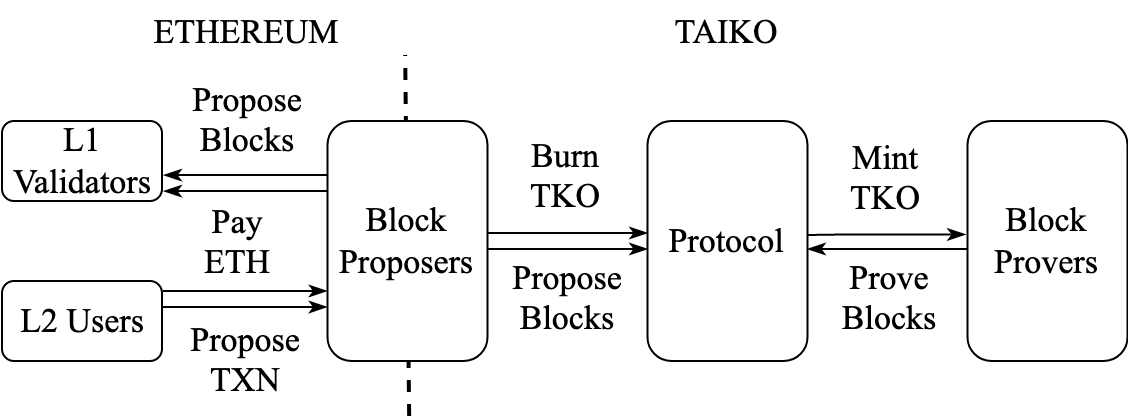
\includegraphics[width=\linewidth]{fig/taikoEcosystemFin2.png}
 \captionof{figure}{The flow of payments, fees and rewards.}
 \label{fig:taiExchange}
 
\end{Figure}


\subsection{Motivation}
We design price dynamics that evolve with respect to a number of different factors (without the use of any price oracles):
\begin{enumerate}
\item The L2 block space. Although block space is much cheaper than on L1, it is still necessary to adjust its price in a way to avoid L2 space being abused. We will enable EIP-1559 on Taiko L2 to dynamically adjust the block space price in a later release (see Section \ref{sec:eip1559-propose}).
\item Protection against external factors, such as TKO token price fluctuations and competing L2 solutions, that can deter proposer and prover engagement with the protocol. Our design enables a dynamic system that introduces fee discounts and reward premiums as incentives, when current engagement falls below average proposal/proof delay statistics. 

\item The current number of unverified blocks. The Taiko protocol has a fixed number of slots, $n_\textnormal{slot}$, for block proposals to allow for parallel proof computation. When there are more unverified blocks occupying the available slots, fees (and rewards) will increase to adjust for the competition within the group of proposers (and similarly for provers).
% (MEV: REMOVED THIS PART BUT HAPPY TO DISCUSS AND INCLUDE WHAT THIS IS TRYING TO SAY.)
% % prevent slots from being over-sold 
% -- this is due to the asynchronous nature of proposals and proofs, therefore, the adjustment of fees and rewards doesn't happen after each block proposal or proof.

\item A system that benefits early-adaptors, working as base discounts for proposal fees that diminish over time, as proposers may be more vulnerable at the initial stages of the protocol compared to provers.
\end{enumerate}

% Our overall fees for proposers and rewards for provers will be a summation of these four components. In this section, we will focus on the last three building blocks.

At the time of submission of a proposal or a proof, referred to as $t$, a proposal fee $f(t)$ or a proof reward $r(t)$ respectively, is calculated as a product of a \textit{base fee} $f_\textnormal{base}$, time-based \emph{incentive multipliers}, $\alpha^+(t)$ and $\alpha^-(t)$, and \emph{slot-availability multipliers}, $\beta^+(n)$ and $\beta^-(n)$, that are based on the number of unverified blocks $n$.
% \begin{align}
% f(t) = f_\textnormal{base} \cdot \beta_\textnormal{icv}^+ \cdot \beta_\textnormal{slot}^+
% \\
% r(t) = f_\textnormal{base} \cdot \beta_\textnormal{icv}^- \cdot \beta_\textnormal{slot}^-
% \end{align}
\begin{align}
f(t) = f_\textnormal{base} \cdot \alpha^+(t) \cdot \beta^+(n)
\\
r(t) = f_\textnormal{base}
\cdot \alpha^-(t) \cdot \beta^-(n)
\end{align}

Although $t$ is determined from the moment of submission of a proof, similar to a proposal, the actual moment of issuing the reward to a prover is potentially much later, when the proof is validated through a series of other proofs that connect it to the genesis block. In other words, proof rewards are determined at the time of submission and minted at the time of validation. 

Throughout the rest of the section, we will use the superscript $^+$ for constants, variables and functions specific to proposals (which add new unverified blocks) and $^-$ for constants, variables and functions specific to proofs (which remove unverified blocks). 

% \subsection{Base Fee}
% The Taiko protocol maintains an internal state variable $f_\textnormal{base}$ called the \textit{Base Fee}. 

% The $f(t)$ dynamics incorporates time based incentives by not discarding them after they are applied but using them to update $f_\textnormal{base}$ through averaging. 
% \subsection{Constants}
% Taiko protocol maintains a number of internal constants $(n, f_\textnormal{base}, t_\textnormal{avg}, t_\textnormal{last})$

\subsection{State Variables}
Taiko protocol maintains a number of internal state variables $(n, f_\textnormal{base}, t^+_\textnormal{ave}, t^-_\textnormal{ave}, t^+_\textnormal{last}, t^-_\textnormal{last})$ that get updated after every successful block proposal or validated proof.
\begin{itemize}
    \item $n$ is the current number of unverified blocks. Initially, $n$ is set to $0$.
    \item $f_\textnormal{base}$ is the base fee, computed as a moving average of its product with incentive multipliers. Initially $f_\textnormal{base}$ is set to a constant $f_\textnormal{init}$.
    \item $t^+_\textnormal{ave}$ is the average duration between proposal submissions conditioned on that they are successful. Initially, $t^+_\textnormal{ave}$ is set to $K_\textnormal{max}^+$.
    % , computed as a moving average of the gap between the current successful submission and the previous successful submission.
    \item $t^-_\textnormal{ave}$ is the average duration between proof submissions conditioned on that they are eventually validated. Initially, $t^+_\textnormal{ave}$ is set to $K_\textnormal{max}^-$.
    % , computed as a moving average of the gap between the current validated submission and the previous validated submission.
    \item $t^+_\textnormal{last}$ is the submission time of the last successful proposal. Initially $t^+_\textnormal{last}$ is set to $0$.
    \item $t^-_\textnormal{last}$ is the submission time of the last validated proof. Initially $t^-_\textnormal{last}$ is set to $0$. 
\end{itemize}
We discuss the state update at the end of the section, after discussing fee and reward computations in a particular state (see Section \ref{sec:priceStateUpdate}). 




% \subsection{Time variables}
% Variables of time are a tuple of three elements: $(t, t_\textnormal{last}, t_\textnormal{ave})$. 
% \begin{itemize}
    
%     \item $t_\textnormal{ave}$ is the average duration between proposals or proofs, computed as a moving average of the gap between $t$ and $t_\textnormal{last}$.
% \end{itemize}


\subsection{Incentive Multipliers}
\label{sec:incentive_mult}
Given a constant $K_\textnormal{inc} > 1$, 
$\alpha^+(t): \mathbb{R}^+\rightarrow [ \nicefrac{1}{K_\textnormal{inc}},1]$ and $\alpha^-(t): \mathbb{R}^+\rightarrow [1, K_\textnormal{inc}] $ are time sensitive multipliers that can decrease fees and increase rewards. 

Their purpose is to incentivize (to a certain degree) proposals and proofs when there are unpredictable deterrents acting against the engagement of proposers or provers, such as imbalances in the pricing that favor one side of the protocol at the expense of the other (internal);  competing L2 marketplaces that offer better deals at the moment or price fluctuations of the TKO token (external).

Incentive multipliers can gradually change the state variable $f_\textnormal{base}$, as will be explained in Section \ref{sec:priceStateUpdate}.

% In order to simplify exposition, in the rest of this section, we drop the superscripts of $t^\textnormal{prop}_\textnormal{ave}, t^\textnormal{proof}_\textnormal{ave}, t^\textnormal{prop}_\textnormal{last}, t^\textnormal{proof}_\textnormal{last}$ and refer to them as $t_\textnormal{ave}, t_\textnormal{last}$ depending on the context, i.e. when computing $\alpha_f(t)$, $t_\textnormal{ave}, t_\textnormal{last}$ will refer to $t^\textnormal{prop}_\textnormal{ave}, t^\textnormal{prop}_\textnormal{last}$ respectively; and when computing $\alpha_r(t)$, $t_\textnormal{ave}, t_\textnormal{last}$ will refer to $t^\textnormal{proof}_\textnormal{ave}, t^\textnormal{proof}_\textnormal{last}$ respectively. 
\subsubsection{Intermediate Time Variables} 
\label{sec:intermediateTimeVar}
% Time-based incentives begin when there is not any successful proposals or proofs for a period longer than 
% a multiple of either; (1) the average duration between proposals or proofs, (2) $T_\textnormal{prop}$ for proposals or $T_\textnormal{proof}$ for proofs.

Given constants $K_\textnormal{grace} \geq 0$,
$K_\textnormal{activation} > 0$, $K^+_\textnormal{max}>0$, $K^-_\textnormal{max}>0$ and state variables, we can compute the following intermediate time variables, $t_\textnormal{grace}$ and $t_\textnormal{activation}$:
\begin{align}
t^+_\textnormal{grace} &\equiv 
 K_\textnormal{grace} \cdot \min(t^+_\textnormal{ave}, K^+_\textnormal{max})\\
t^-_\textnormal{grace} &\equiv K_\textnormal{grace} \cdot \min(t^-_\textnormal{ave}, K^-_\textnormal{max}).
\end{align}
% \begin{align}
%     t_\textnormal{grace} \equiv 
%  \begin{dcases}
%  K_\textnormal{grace} \cdot \min(t^+_\textnormal{ave}, K^+_\textnormal{max}), &\text{if a \emph{proposal}} \\
% K_\textnormal{grace} \cdot \min(t^-_\textnormal{ave}, K^-_\textnormal{max}), &\text{if a \emph{proof}}
% \end{dcases}
% \end{align}
% or, omitting the superscripts,
% \begin{align}
%     t_\textnormal{grace} \equiv 
%  K_\textnormal{grace} \cdot \min(t_\textnormal{ave}, K_\textnormal{max}).
% \end{align}
% \begin{align}
% t_\textnormal{grace}  \equiv  K_\textnormal{GracePeriod} \cdot \min(t^\textnormal{proof}_\textnormal{ave}, K_\textnormal{BlockTimeCap})
% \end{align}
$t_\textnormal{grace}$ is the grace period starting at $t_\textnormal{last}$ (omitting the superscript) in which there are no incentives yet.
% do not activate and $f_\textnormal{min}$ remains unchanged. It is related to $t_\textnormal{ave}$ through $t_\textnormal{grace} = k_{\textnormal{grace}} \cdot t_\textnormal{ave}$.
% \begin{align}
%     t_\textnormal{max} \equiv 
%  \begin{dcases}
%  K_\textnormal{max} \cdot \min(t^\textnormal{prop}_\textnormal{ave}, T_\textnormal{prop}), &\text{if a \emph{proposal}} \\
% K_\textnormal{max} \cdot \min(t^\textnormal{proof}_\textnormal{ave}, T_\textnormal{proof}), &\text{if a \emph{proof}}
% \end{dcases}
% \end{align}
% \begin{align}
% t_\textnormal{activation} \equiv 
%  K_\textnormal{activation} \cdot \min(t_\textnormal{ave}, K_\textnormal{max}).
% \end{align}
\begin{align}
t^+_\textnormal{activation} &\equiv 
 K_\textnormal{activation} \cdot \min(t^+_\textnormal{ave}, K^+_\textnormal{max})\\
t^-_\textnormal{activation} &\equiv 
 K_\textnormal{activation} \cdot \min(t^-_\textnormal{ave}, K^-_\textnormal{max}).
\end{align}
% \begin{align}
% t_\textnormal{max}  \equiv   K_{\mathrm{MaxPeriod}} \cdot \min(t_\textnormal{ave}, K_\textnormal{ProofTimeCap}) 
% \end{align}

$t_\textnormal{activation}$ is the time period after which incentives reach their maximum effects from the time they first start to take effect at $t_\textnormal{last}+t_\textnormal{grace}$ (omitting the superscripts). 
\begin{Figure}
 \centering
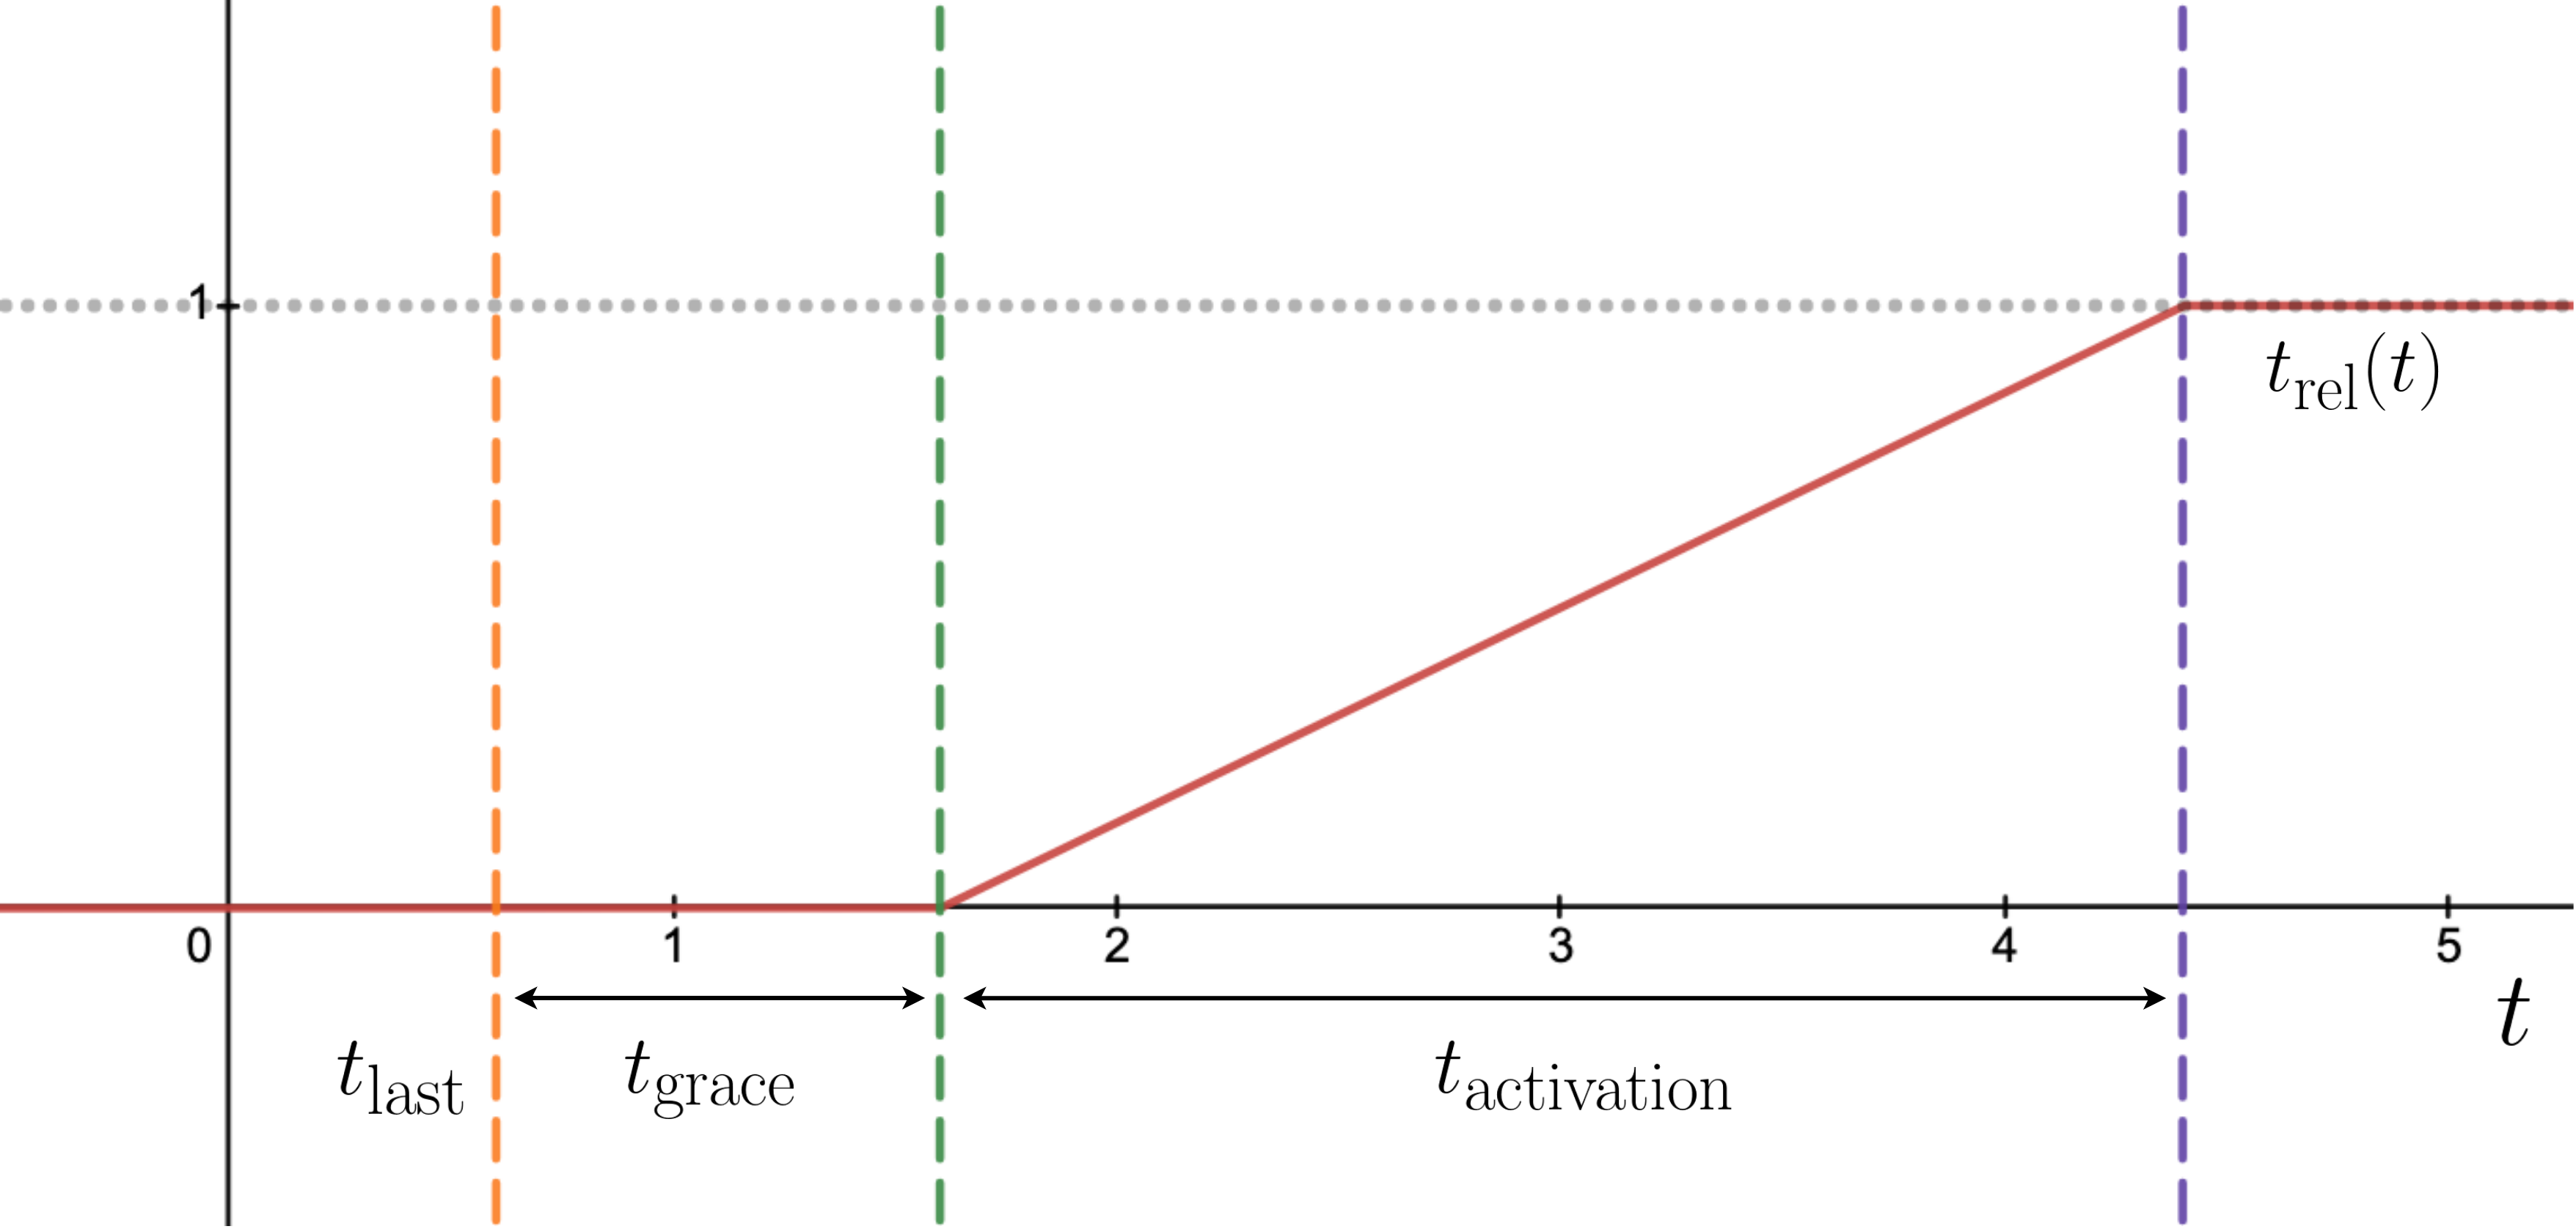
\includegraphics[width=0.9\linewidth]{fig/relative_time_graph.png}
 % \vspace{-0.2in}
 \vspace{-0.1in}
 \captionof{figure}{The graph of $t_\textnormal{rel}$ (red) with respect to time $t$ given $t_\textnormal{last}$, $t_\textnormal{grace}$, $t_\textnormal{activation}$ (omitting the superscripts).}
\label{fig:relativetime}
\end{Figure}

Two functions of note are $t^+_\textnormal{rel}(t),t^-_\textnormal{rel}(t): \mathbb{R}^+ \rightarrow [0,1]$ and they are defined as
\begin{align}
t_\textnormal{rel}^+(t) &=  
% \frac{\textnormal{min}(\textnormal{max}(0, t - (t_{\textnormal{last}} + t_{\textnormal{grace}})), t_{\textnormal{max}})}{t_{\textnormal{max}}} 
\textnormal{min}\left(\textnormal{max}\left(0, \frac{t - (t^+_\textnormal{last} + t^+_\textnormal{grace})}{t^+_\textnormal{activation}}\right), 1\right)\\
t_\textnormal{rel}^-(t) &=  
% \frac{\textnormal{min}(\textnormal{max}(0, t - (t_{\textnormal{last}} + t_{\textnormal{grace}})), t_{\textnormal{max}})}{t_{\textnormal{max}}} 
\textnormal{min}\left(\textnormal{max}\left(0, \frac{t - (t^-_\textnormal{last} + t^-_\textnormal{grace})}{t^-_\textnormal{activation}}\right), 1\right)
.
\end{align}

$t_\textnormal{rel}$ indicates \emph{relative normalized time}, and determines the activation point of time-based incentives, where $t_\textnormal{rel}$ becomes greater than $0$, and the saturation point of incentives, where $t_\textnormal{rel}$ becomes equal to $1$ (see Figure \ref{fig:relativetime}).

\begin{Figure}
 \centering
 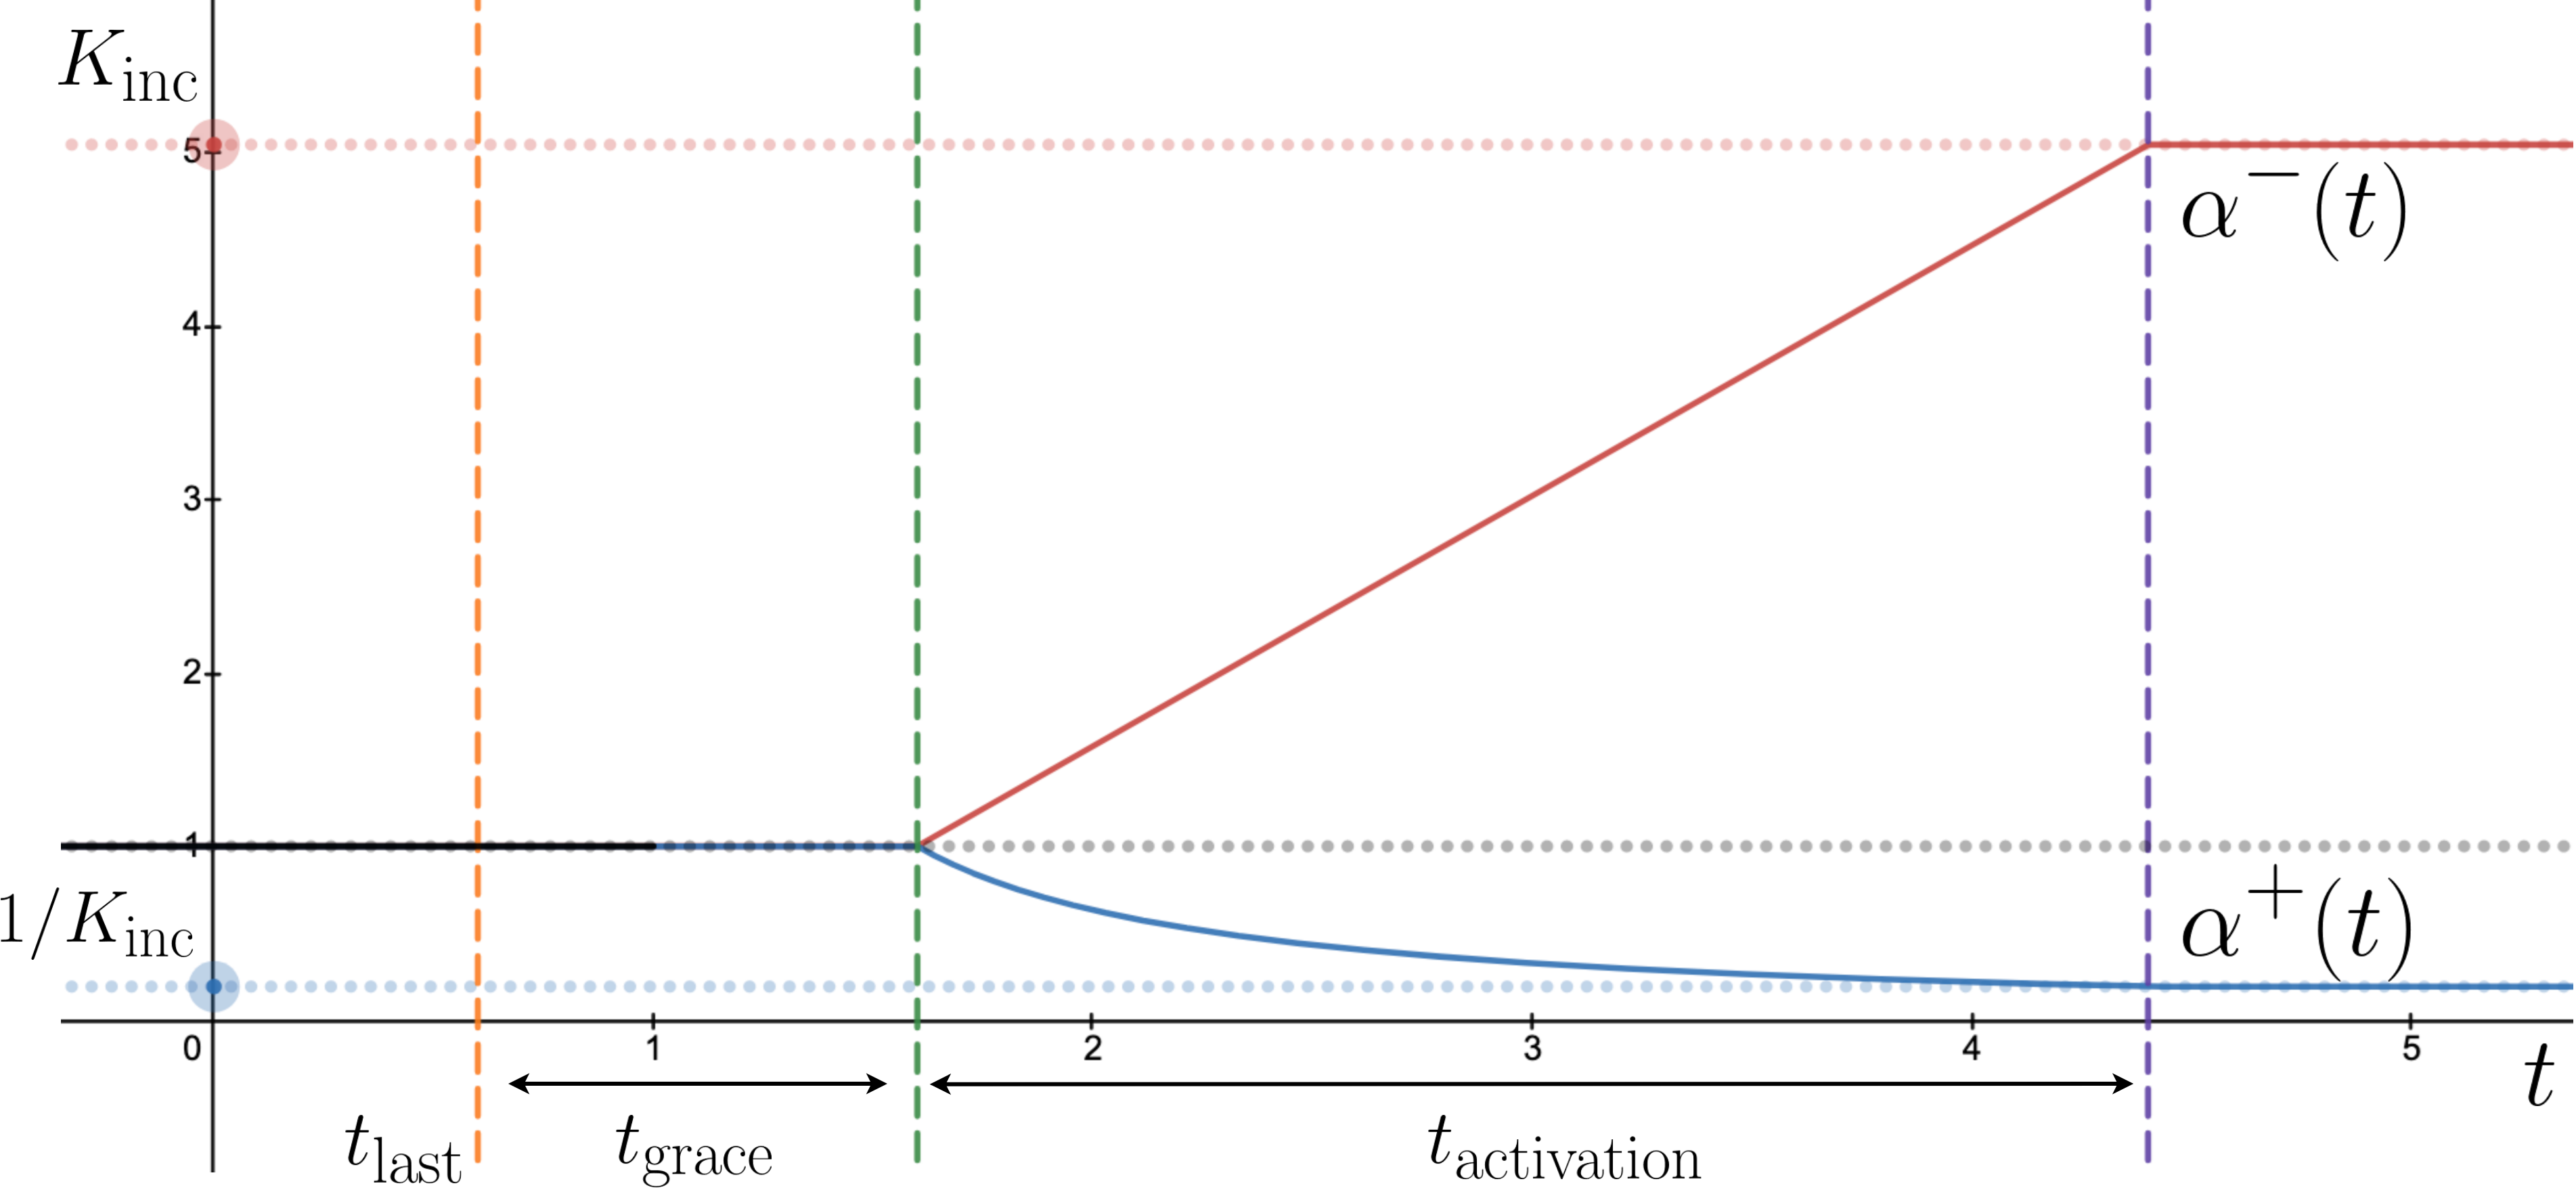
\includegraphics[width=0.9\linewidth]{fig/incentive_graph.png}
 \captionof{figure}{The graphs of $\alpha^+(t)$ (blue) and $\alpha^-(t)$ (red), which are multiplicative inverses of each other if $t^+_\textnormal{rel}(t)=t^-_\textnormal{rel}(t)$.}
\label{fig:incentive_multiplier_graphs}
\end{Figure}
\subsubsection{Multipliers}
% Parameters of incentives and averaging computations are $\{\alpha, \mu, t_\textnormal{init}, f_\textnormal{init}\}$. 
Given the constant $K_\textnormal{inc}$  % does not make sense to initialize it as this is not a variable, we can just change all the constants to K_something later if desired.
% (initialized as $K_{\mathrm{RewardMultiplier}}$)
and the relative normalized time functions $t^+_\textnormal{rel}(t), t^-_\textnormal{rel}(t)$ established using state variables, we compute incentive multipliers $\alpha^+(t)$, $\alpha^-(t)$ as
\begin{align}
% \beta & \equiv  1 + (\alpha - 1)\cdot t_\textnormal{rel}(t, t_\textnormal{last},
%  t_\textnormal{avg})\\
% % \end{align}
% % \begin{align}
% \Gamma_\textnormal{inc}(t, t_\textnormal{last},
%  t_\textnormal{avg}) & \equiv 
%  \begin{dcases}
%     \frac{1}{\beta}, &\text{if a \emph{proposal}} \\
%      \beta, &\text{if a \emph{proof}}
% \end{dcases}
\alpha^+(t) &= \nicefrac{1}{1 + (K_\textnormal{inc} - 1)\cdot t_\textnormal{rel}^+(t)}\\
\alpha^-(t) &= 1 + (K_\textnormal{inc} - 1)\cdot t_\textnormal{rel}^-(t). 
\end{align}
% We initialize $t_\textnormal{last} \equiv 0$ , $t_\textnormal{ave} \equiv t_\textnormal{init}$ and $f_\textnormal{avg}\equiv f_\textnormal{init}$. $\alpha$ is the maximum incentive ratio. $\mu$ is the momentum parameter for the moving average (higher $\mu$ makes the effects of individual updates smaller). $t_\textnormal{init}$ is the initial time gap average before any transactions. $f_\textnormal{init}$ is the initial multiplier for slot based prices.
% At every new transaction at time $t$, we compute the following in sequence: 
% \begin{align}
% \beta & \equiv  1 + (\alpha - 1)\cdot t_\textnormal{rel}(t, t_\textnormal{last},
%  t_\textnormal{avg})\\
% % \end{align}
% % \begin{align}
% \Gamma_\textnormal{inc}(t, t_\textnormal{last},
%  t_\textnormal{avg}) & \equiv 
%  \begin{dcases}
%     \frac{1}{\beta}, &\text{if a \emph{proposal}} \\
%      \beta, &\text{if a \emph{proof}}
% \end{dcases}
% \end{align}
% As shown by the figure below, the proposing fee can be reduced to $\nicefrac{f_\textnormal{b}}{\alpha}$, and the proving reward can be amplified up to $f_\textnormal{b} \cdot \alpha$.
As shown in Figure \ref{fig:incentive_multiplier_graphs}, the incentive multiplier for proof rewards, $\alpha^-(t)$, cannot exceed $K_\textnormal{inc}$ and the incentive multiplier for proposal fees, $\alpha^+(t)$, cannot be less than $\nicefrac{1}{K_\textnormal{inc}}$.

\subsection{Slot-availability Multipliers}
\label{sec:slot_availability_multipliers}
% Removing this part for now, as it is not quite there (it introduces new variables not well defined and are not used directly). I will consider this reasoning later on and see if it can be added on. 
% The expected number of unverified blocks is $\nicefrac{t^\textnormal{p}_\textnormal{ave}}{t^\textnormal{b}_\textnormal{ave}}$, where $t^\textnormal{b}_\textnormal{ave}$ is the average block proposal time and $t^\textnormal{p}_\textnormal{ave}$ is the average proof delay. 
% When the number of unverified blocks is smaller than expected, the proposing fee shall be reduced to encourage block proposals; otherwise the proof reward shall be increased to encourage prover engagement. 
% Instead of relying on the comparison with $\nicefrac{t^\textnormal{p}_\textnormal{ave}}{t^\textnormal{b}_\textnormal{ave}}$, this can be accomplished using the \emph{constant-product} pricing mechanism as used by Uniswap V1. 
Slot-availability multipliers are computed solely from the current number of unverified blocks $n$ and they are independent of time given a particular state. 

These multipliers capture the idea of offering the lowest fees and rewards when there are only a few unverified blocks and a surplus of available slots, $n_\textnormal{slots}-n$. In this case, parallel proof computation can accommodate many proposers, which leads to low competition and consequently lower fees. Further, there is a shortage of unverified blocks to prove, which means that provers must compete with each other to get the rewards (which allows lower rewards). 

In the opposite case, the level of competition for proposers and provers are reversed when there are many unverified blocks. As the number of available slots, $n_\textnormal{slots}-n$, decrease, competition for the remaining slots increase for proposers, which leads to higher fees. Further, since there are many unverified blocks, competition for provers is low, which results in higher rewards. 

% In the opposite case of many unverified blocks, fees are higher as new proposers must compete to get the last few available slots. Similarly, the rewards are higher because there are plenty of unverified blocks to go around for provers. 

Therefore, fees and rewards increase as the number of unverified blocks grow, through multipliers $\beta^+(n)$ and $\beta^-(n)$ respectively, which are governed by a 
% \emph{constant-product}
pricing mechanism used in Uniswap V1, described below.

Given a smoothing constant $K_\textnormal{slot} \geq 1$ that determines how slowly the slot-availability multipliers increase as $n$ grows, 
% another constant, $\Phi$, is computed from $n_\textnormal{slots}$ and $\lambda$.
% \begin{align}
%     % \Phi \equiv \underbrace{(n_\textnormal{slots} + \lambda - 1)}_{k(t=0)} \cdot \underbrace{(n_\textnormal{slots} + \lambda)}_{n_\textnormal{slots}-n(t=0) + \lambda}\\
%     \Phi \equiv (n_\textnormal{slots}- 1 + \lambda ) \cdot (n_\textnormal{slots} + \lambda)
% \end{align}
% This invariant remains the same across all time, as the number of available slots $n(t)$ changes by $m$ blocks due to successful proposals and proofs: 
% \begin{align}
%     \Phi(t) \equiv k(t, m) \cdot (n(t) + \lambda + m) \equiv \Phi
% \end{align}
% This requires that $k(t, m) \equiv \nicefrac{\Phi}{n(t) + \lambda} + m$. Therefore, $k(t, m)$ at any given time follows an inverse law with respect to available slots $n(t)$. 
% At any given time point $t$, we can update the fee or reward $f(t)$ as:
% \pagebreak
we define $\beta^+(n): \{n\in \mathbb{Z} \hspace{0.02in}|\hspace{0.02in}  0 \leq n < n_\textnormal{slots} \}\rightarrow \mathbb{R}^+$ and $\beta^-(n): \{n\in \mathbb{Z} \hspace{0.02in}|\hspace{0.02in}  0 < n \leq n_\textnormal{slots} \}\rightarrow \mathbb{R}^+$ as, 

% \begin{align}
% \beta_f(n) &= \frac{\Phi}{(n_\textnormal{slots}-n-1 + \lambda)\cdot (n_\textnormal{slots}-n + \lambda)}\\
% \beta_r(n) &= \frac{\Phi}{(n_\textnormal{slots}-n + 1 + \lambda)\cdot (n_\textnormal{slots}-n + \lambda)}
% \end{align}

\begin{align}
n'_\textnormal{slots} &= n_\textnormal{slots} + K_\textnormal{slot} \\
\beta^+(n) &= \frac{(n'_\textnormal{slots}- 1) \cdot n'_\textnormal{slots}}{(n'_\textnormal{slots}-n-1)\cdot (n'_\textnormal{slots}-n)}\\
\beta^-(n) &= \frac{(n'_\textnormal{slots}- 1 ) \cdot n'_\textnormal{slots}}{(n'_\textnormal{slots}-n + 1)\cdot (n'_\textnormal{slots}-n)}.
\end{align}
% (n_\textnormal{slots}- 1 + \lambda ) \cdot (n_\textnormal{slots} + \lambda)
% \begin{align}
% m & \equiv & 
% \begin{dcases}
%    -1, & \text{if a \emph{proposal}} \\
%     1, & \text{if a \emph{proof}} \\
% \end{dcases}\\
% f^*(t) & \equiv & f(t) \cdot  \left\lvert k(t, 0) - k(t, m)\right\lvert \\
% \nonumber& \equiv & f(t) \cdot \left\lvert \frac{\Phi}{n(t) + \lambda}-\frac{\Phi}{n(t) + \lambda + m}\right\lvert \\
% \nonumber & \equiv & f(t) \cdot  \frac{\Phi}{(n(t) + \lambda + m)\cdot (n(t) + \lambda)}
% \end{align}
It is easy to see that for $n=0$, which corresponds to the case of not having any unverified blocks, the multiplier for fees is
% \begin{align}
% \beta_f(0) &= \frac{\Phi}{(n_\textnormal{slots}-1 + \lambda)\cdot (n_\textnormal{slots} + \lambda)}=1
% \end{align}
\begin{align}
\beta^+(0) &= \frac{(n'_\textnormal{slots}- 1 ) \cdot n'_\textnormal{slots}
}{(n'_\textnormal{slots}-1)\cdot n'_\textnormal{slots}}=1.
\end{align}
% (n_\textnormal{slots}- 1 + \lambda ) \cdot (n_\textnormal{slots} + \lambda)
% simply from the definition of $\Phi$.
In this case, the overall fee simplifies to
\begin{align}
f(t) = f_\textnormal{base} \cdot \alpha^+(t).
\end{align}

Further, if $n = n_\textnormal{slots}-1$ (only one slot is available),  the multiplier for fees takes its maximum value,
\begin{align}
\beta^+(n_\textnormal{slots}-1)
% &= \frac{\Phi}{(\lambda)\cdot (1 + \lambda)} \\
% \nonumber 
&= 
\frac{(n_\textnormal{slots}- 1 + K_\textnormal{slot} ) \cdot (n_\textnormal{slots} + K_\textnormal{slot})}{K_\textnormal{slot}\cdot (1 + K_\textnormal{slot})}.
\end{align}

Finally, we note that for all valid inputs $\{n\in \mathbb{Z} \hspace{0.02in}|\hspace{0.02in}  0 \leq n < n_\textnormal{slots} \}$,
\begin{align}
    \beta^-(n+1) = \beta^+(n)
\end{align}
which ensures that the multiplier of the reward for a proven block equals the multiplier for its fee when it was proposed.

% \begin{align}
% f^*(t)  & \equiv & f(t) \cdot \frac{\Phi}{\lambda\cdot (1+\lambda)} \\
% \nonumber & \equiv & f(t) \cdot \frac{(n_\textnormal{max} + \lambda - 1) \cdot (n_\textnormal{max} + \lambda)}{\lambda\cdot (1+\lambda)}
% \end{align}

% If we hold $f(t)$ constant, the ratio between the last and the first slot's proposal fee is, 
% \begin{align}
% % \frac{f(1)}{f(n_{\textnormal{max}})} = 
% R  \equiv \frac{(n_\textnormal{max} + \lambda - 1) \cdot (n_\textnormal{max} + \lambda)}{\lambda\cdot (1+\lambda)}.
% \end{align}

\begin{Figure}
 \centering
 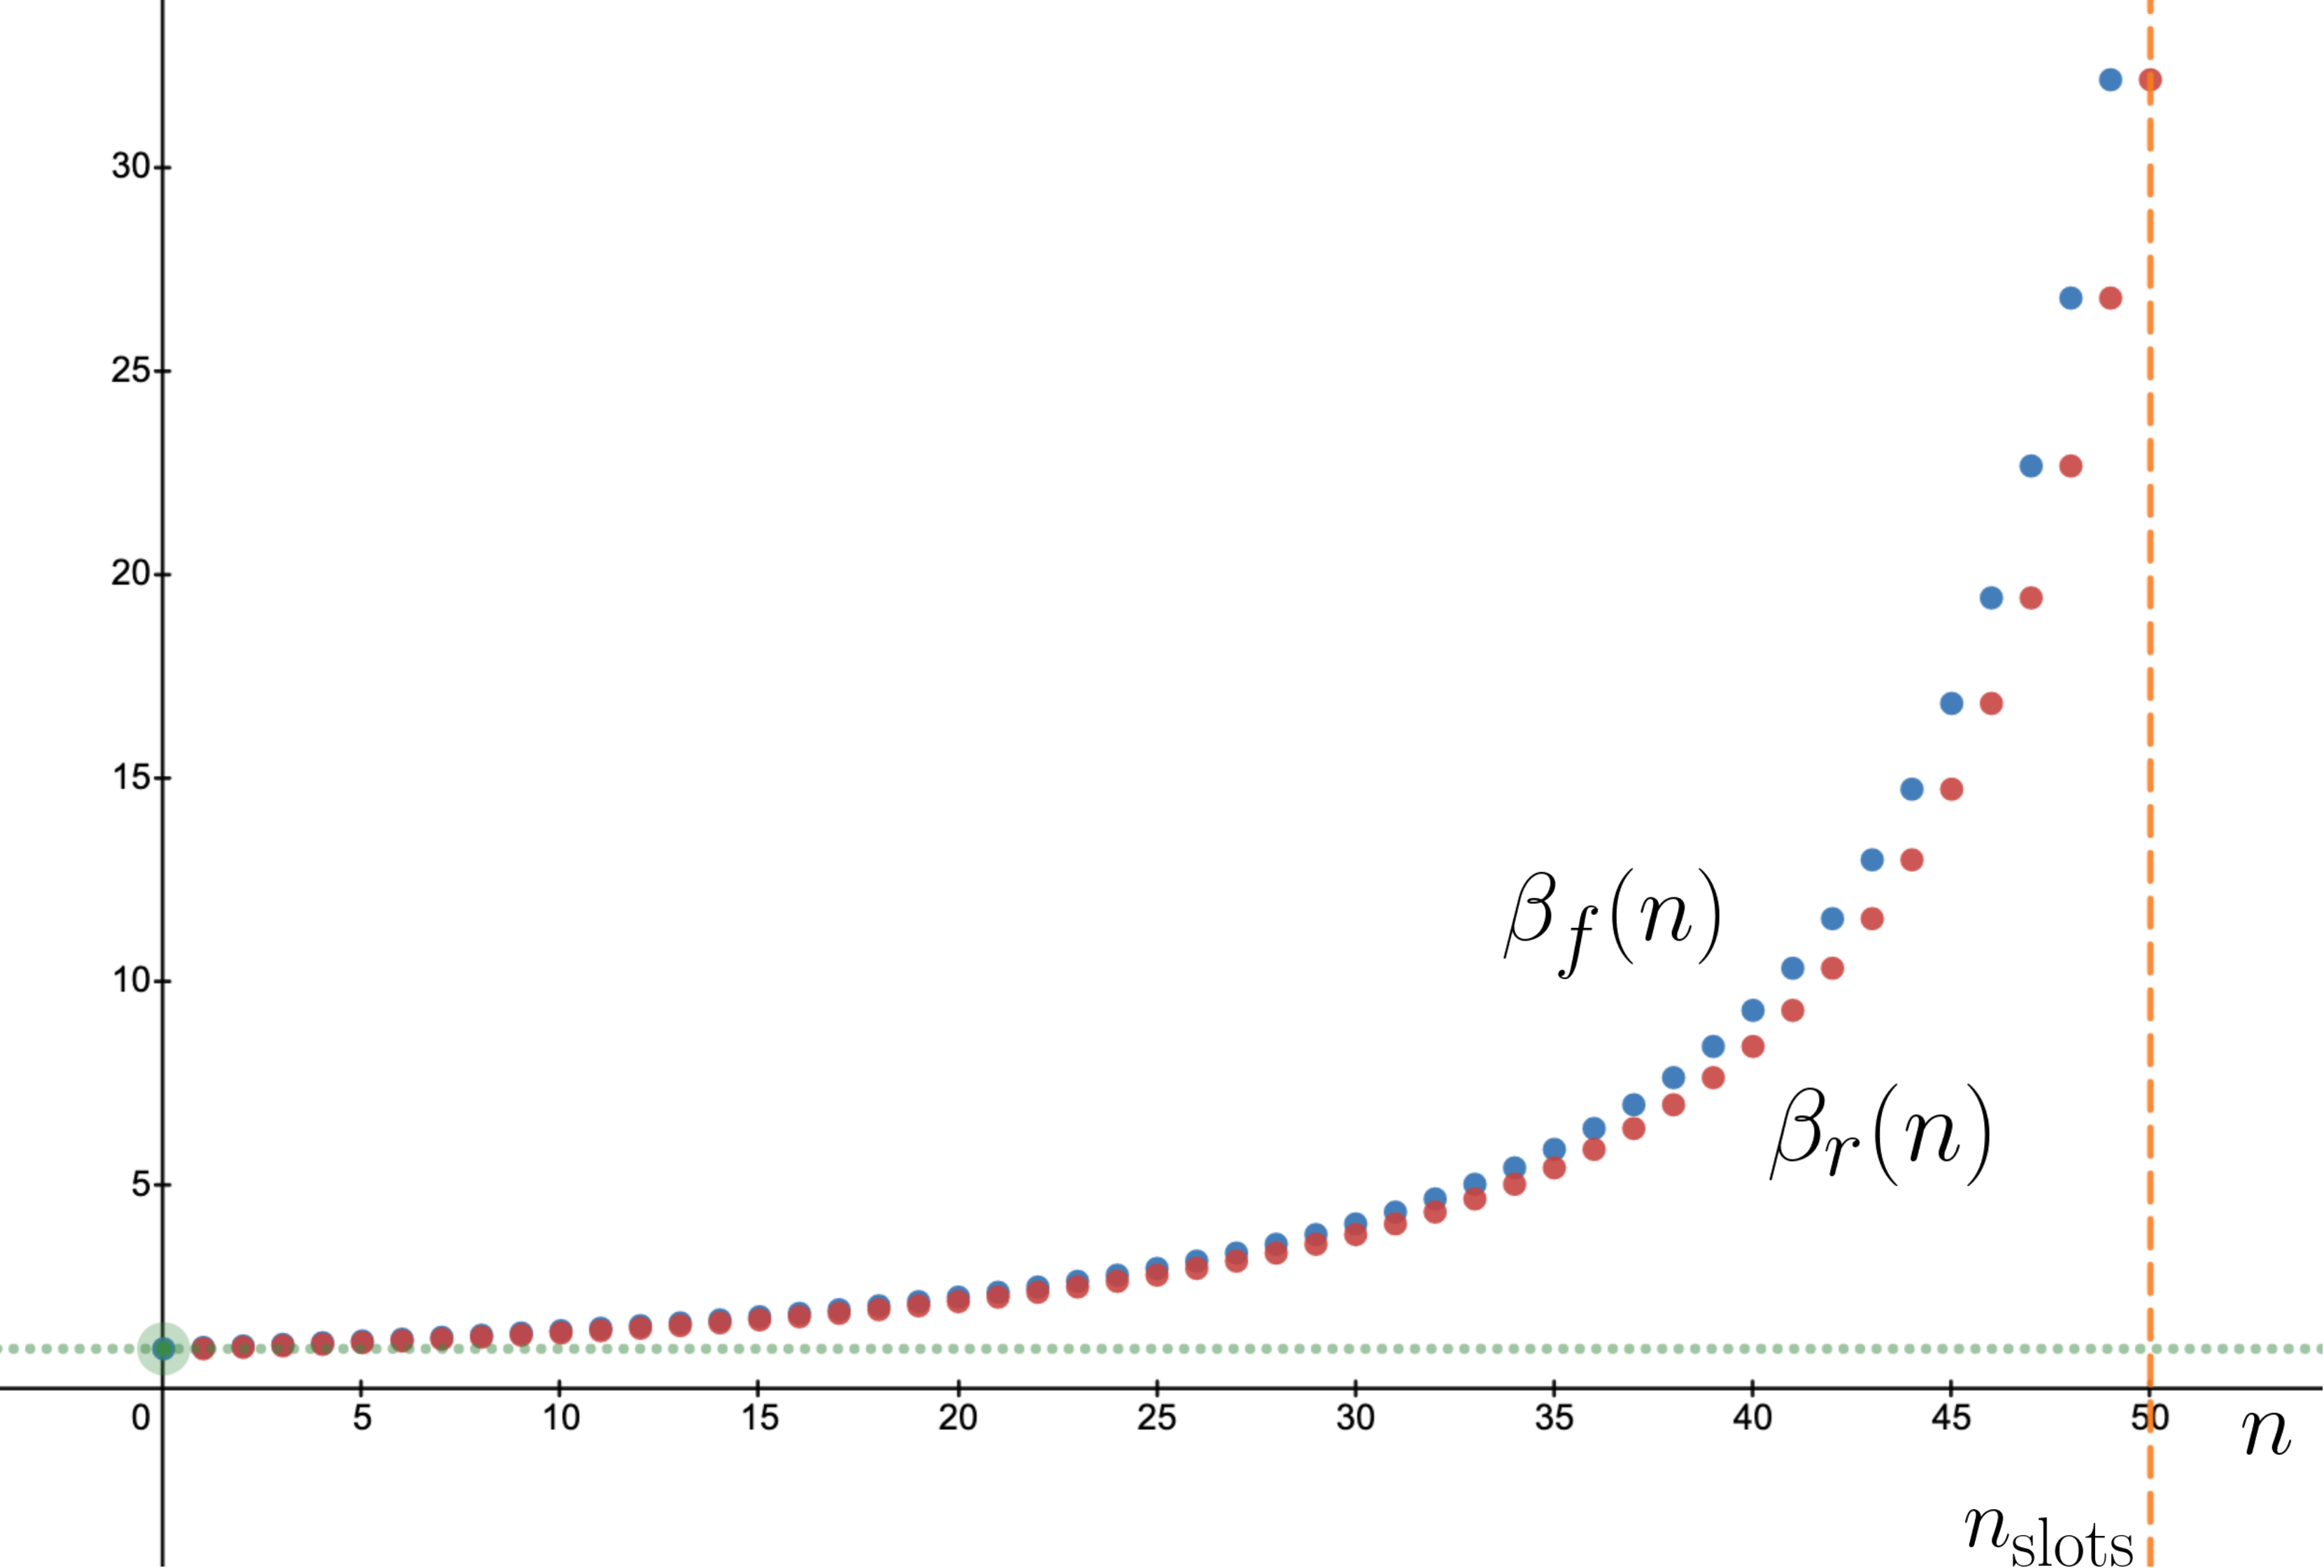
\includegraphics[width=0.8\linewidth]{fig/lambda10.png}
 \captionof{figure}{Progression of the multiplier for fees $\beta^+(n)$ (blue) and the multiplier for rewards $\beta^-(n)$ (red), when $n_{\textnormal{slots}}=50$ and $K_\textnormal{slot}=10$. The maximum value of the multiplier is $\frac{(n_\textnormal{slots} - 1 + K_\textnormal{slot} ) \cdot (n_\textnormal{slots} + K_\textnormal{slot})}{K_\textnormal{slot}\cdot (1+K_\textnormal{slot})}=32.182$.}
 \label{fig:f_slot_lambda1}
\end{Figure}

Finally, in Figures \ref{fig:f_slot_lambda1} and \ref{fig:f_slot_lambda50}, we demonstrate that the smoothing term $K_\textnormal{slot}$ can be increased to attenuate the maximum value of slot-availability multipliers.

\begin{Figure}
 \centering
 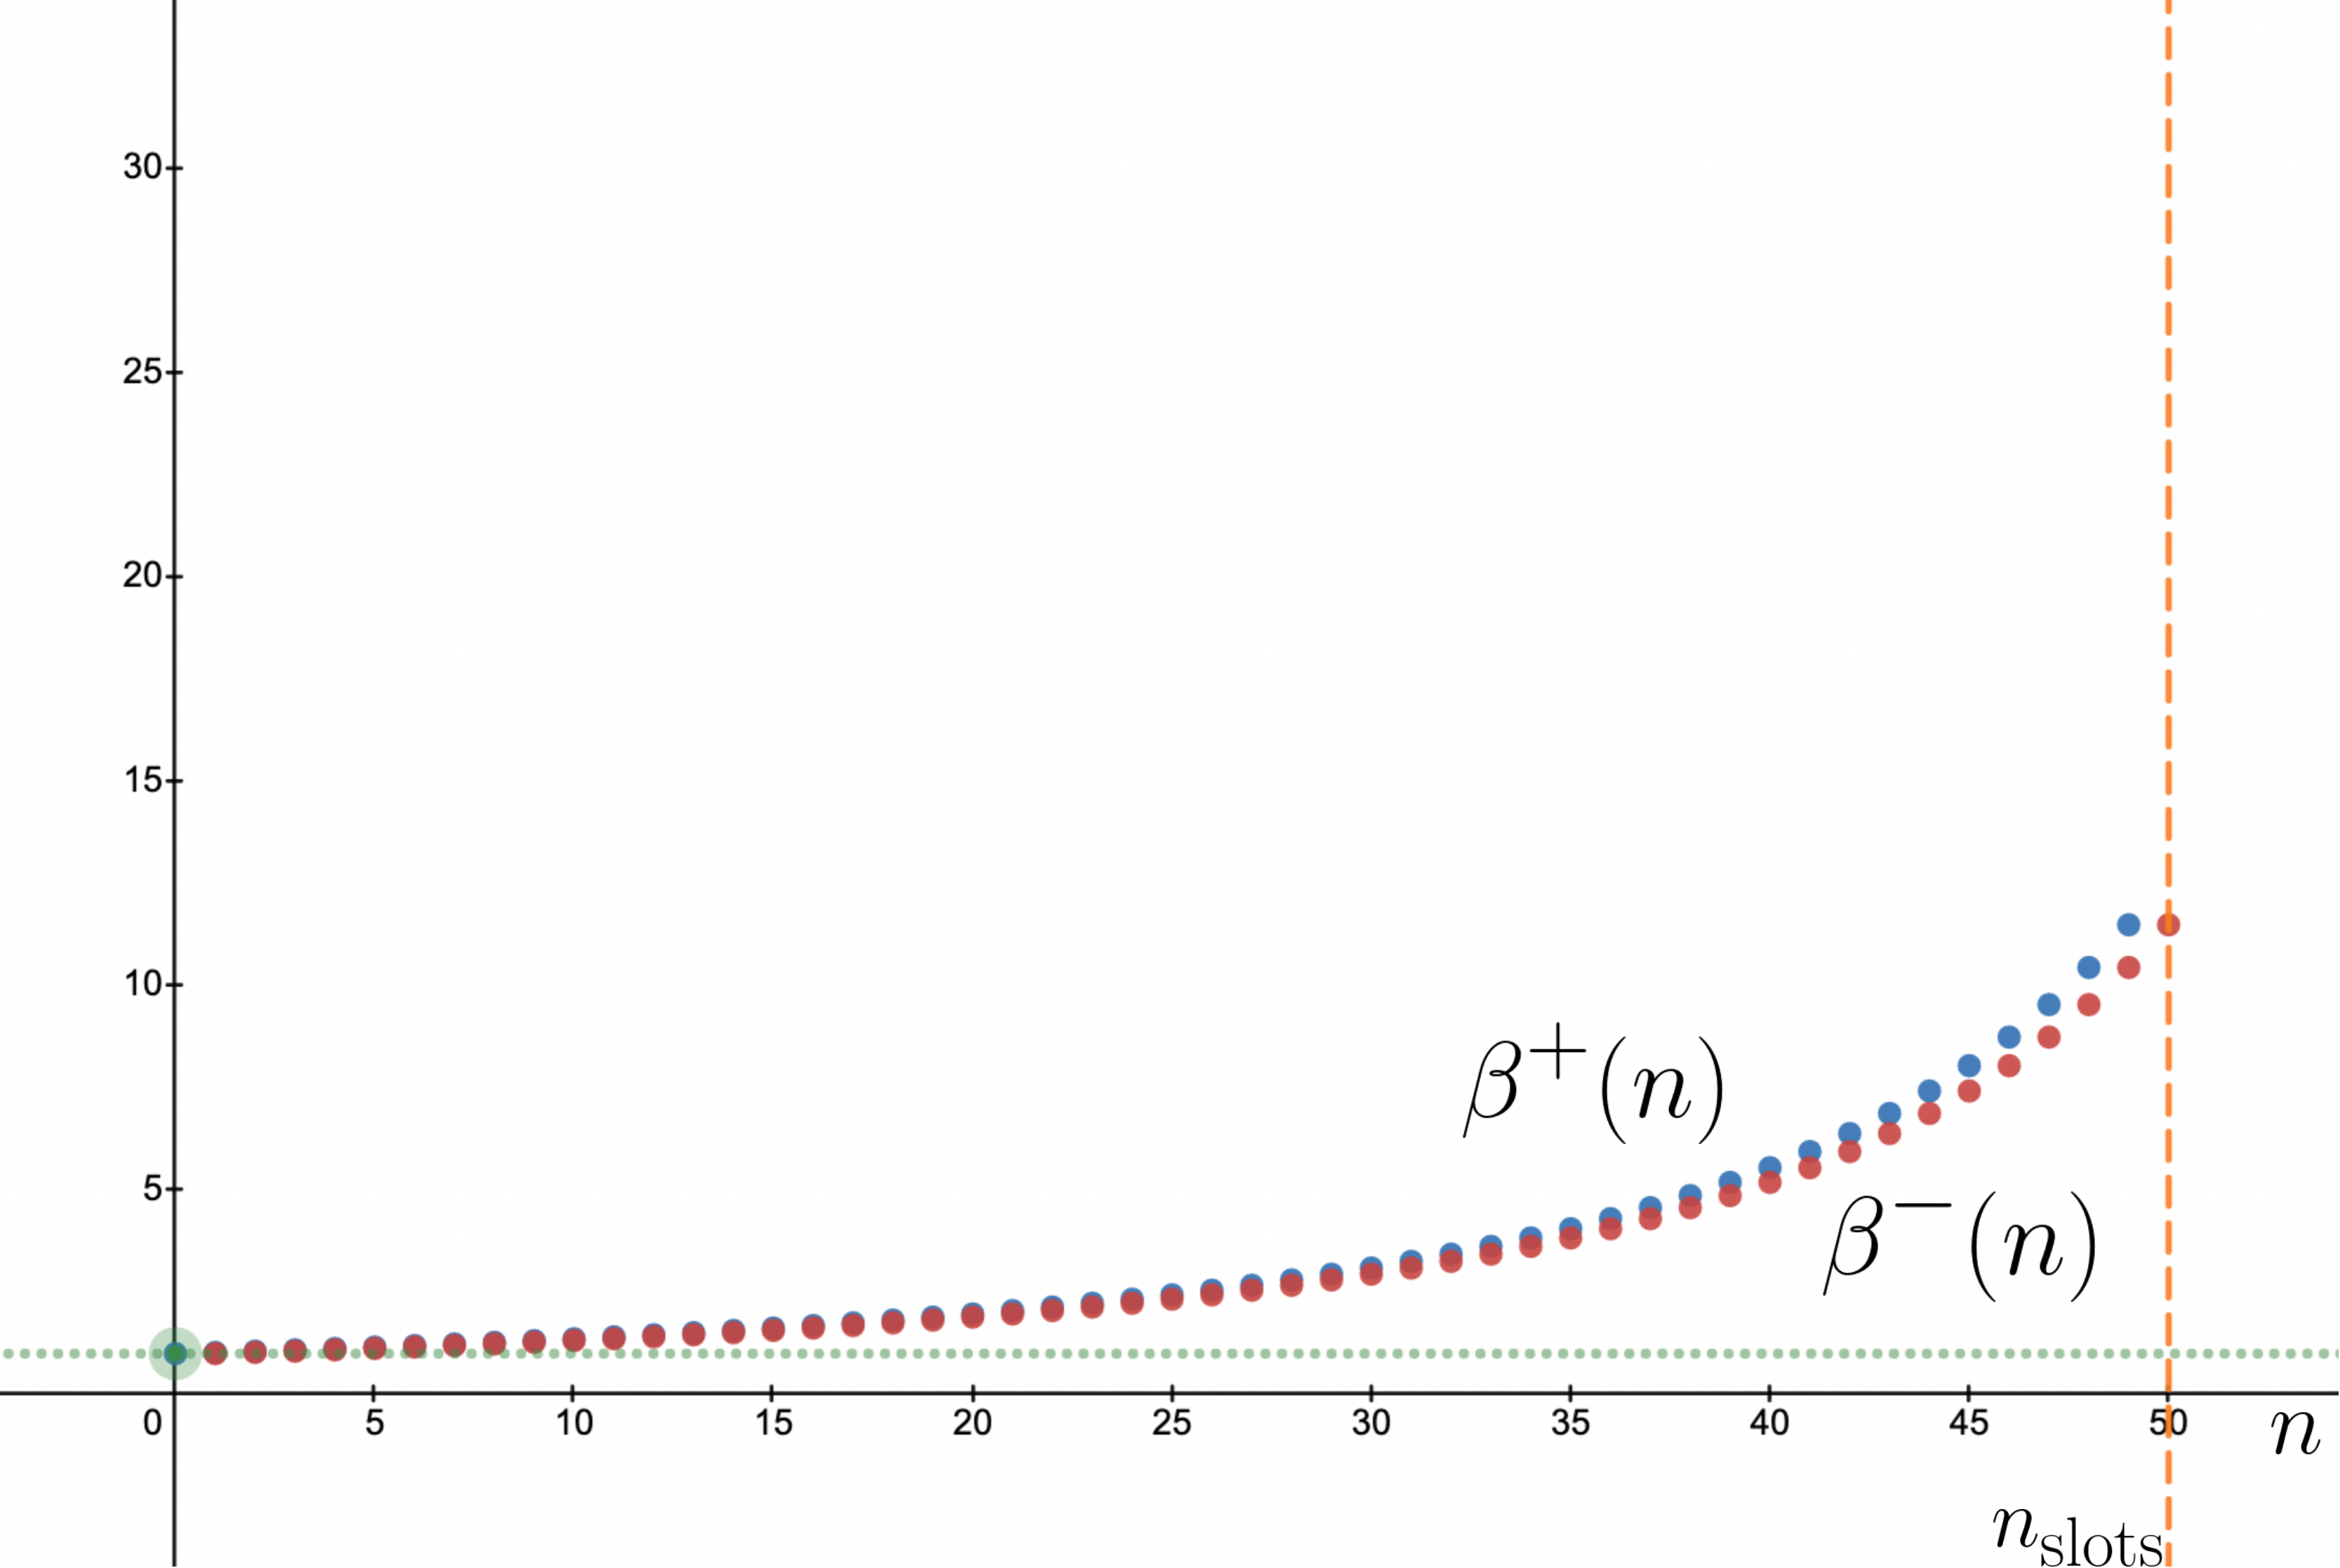
\includegraphics[width=0.8\linewidth]{fig/lambda20.png}
 \captionof{figure}{Progression of the multiplier for fees $\beta^+(n)$ (blue) and the multiplier for rewards $\beta^-(n)$ (red), when $n_{\textnormal{slots}}=50$ and $K_\textnormal{slot}=20$. The maximum value of the multiplier is $\frac{(n_\textnormal{slots} - 1 + K_\textnormal{slot} ) \cdot (n_\textnormal{slots} + K_\textnormal{slot})}{K_\textnormal{slot}\cdot (1+K_\textnormal{slot})}=11.5$.}
 \label{fig:f_slot_lambda50}
 
\end{Figure}

\subsection{Bootstrap Discount Multipliers}\label{sec:bootstrapping}
Unlike block provers, proposers are directly affected by the number of active L2 users, as well as ETH fees they need to pay to the L1-layer validators. This makes them vulnerable at the initial stages of the protocol when there are not many L2 users engaging it with their transactions, which makes it hard for proposers to create larger and more profitable blocks with many transactions in them.

\begin{Figure}
 \centering
 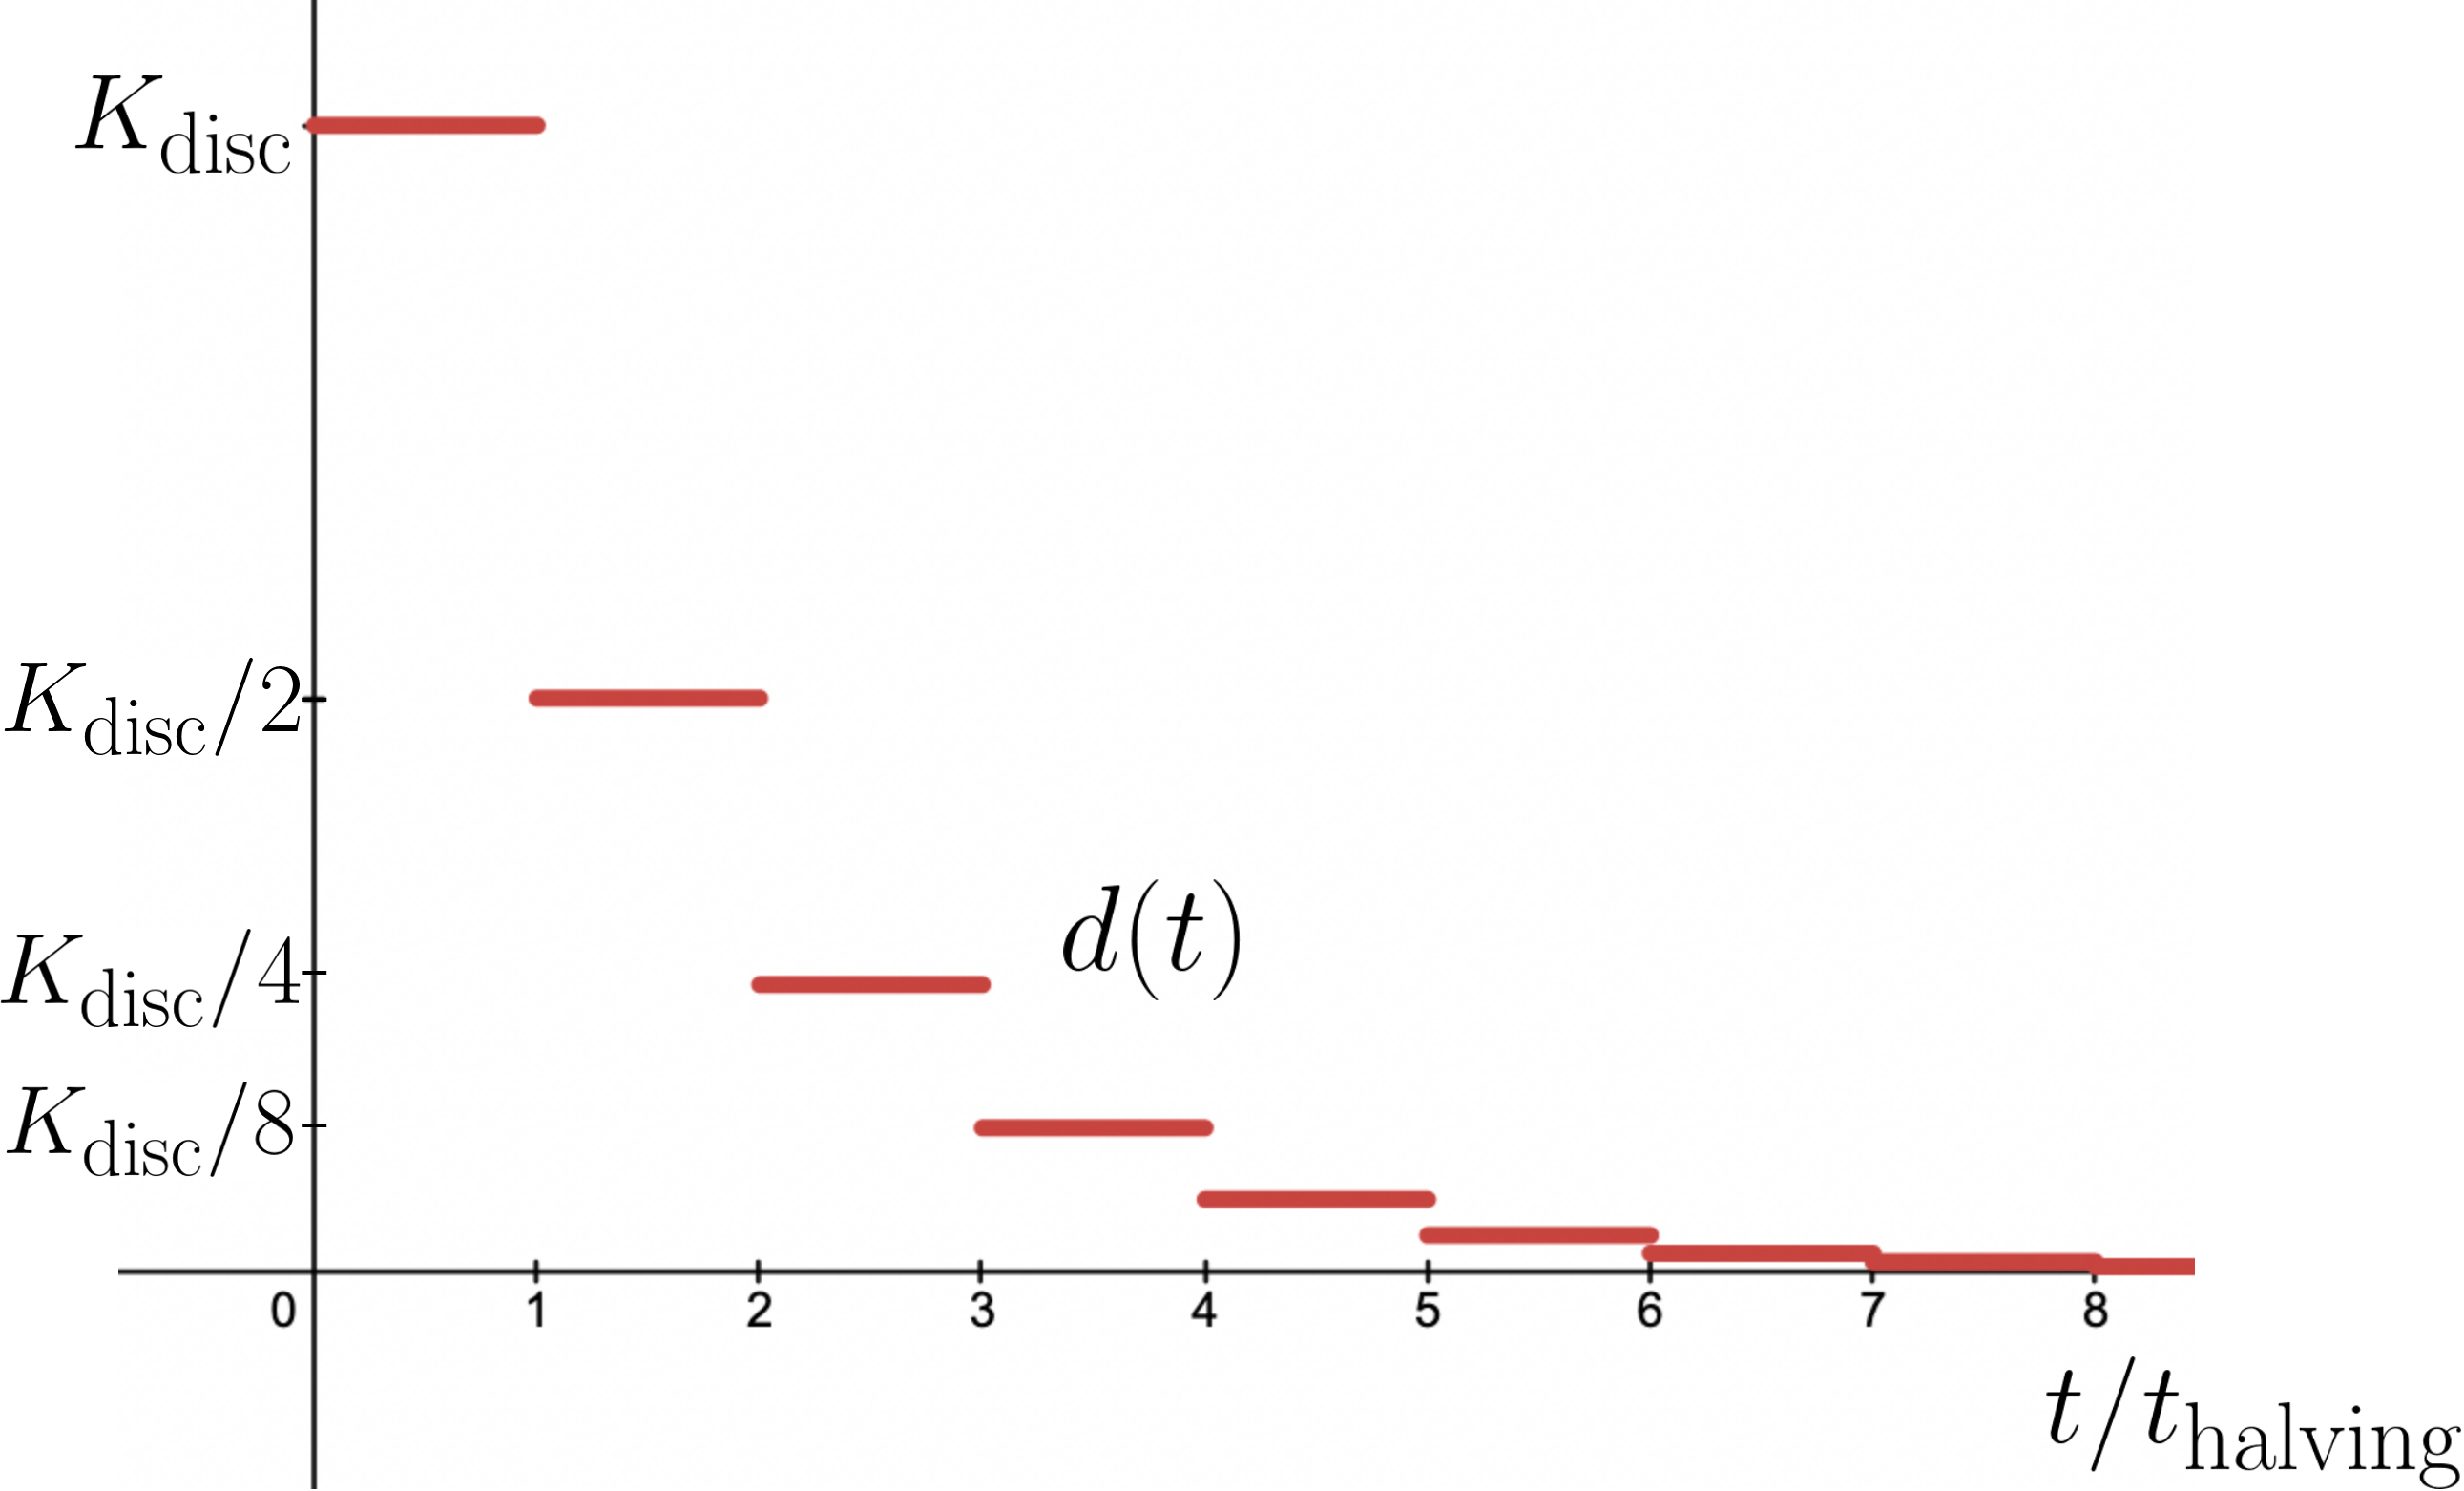
\includegraphics[width=0.8\linewidth]{fig/discount_func.png}
 \captionof{figure}{Graph of discount function $d(t)$.}
 \label{fig:discount}
\end{Figure}

Given an initial discount rate constant $K_\textnormal{disc} \in (0, 1]$ and a halving period constant $K_\textnormal{Halving} > 0$, we can compute a discount function $d(t)$ and a discount multiplier for fees $\gamma^+(t)$ as functions of time:

\begin{align}
d(t) &= K_\textnormal{disc}\cdot (\nicefrac{1}{2})^{\lfloor \nicefrac{t}{K_\textnormal{Halving}}\rfloor}
\\
\gamma^+(t)  &= 1-d(t).
\end{align}

As time passes, this multiplier approaches $1$, which means that its effects diminish over time.

The discount multiplier is applied to the overall proposal fee computation as follows: 
% 
% During the bootstrapping period after the network goes live, block proposers may not be able to collect enough transactions to justify their proposing fees. Therefore, a dedicated pool of TKO token, $B = K_{\mathrm{BootstrapReward}}$, is set up to reward early block proposers over a period $T = K_{\mathrm{BootstrapPeriod}}$ so they are willing to keep proposing smaller blocks.
% 
% For each block, the bootstrapping reward $r(t)$ is calculated as


% \begin{eqnarray}
% \\
% \nonumber r(t) \equiv
%  \begin{dcases}
%     \frac{(T - t_\textnormal{last})^2 - (T - t)^2}{T^2} \cdot B, &\text{if} \quad t < T \\
%     0, &\text{otherwise}
% \end{dcases}
% \end{eqnarray}

% The larger the gaps between $t_\textnormal{last}$ and $t$ is, the larger the bootstrapping reward will be.

\begin{align}
f(t) = f_\textnormal{base} \cdot \alpha^+(t) \cdot \beta^+(n) \cdot \gamma^+(t)
\end{align}

Bootstrapping support is applicable only to proposer fees in order to safeguard the normal market order conditions between proposers and provers.

\subsection{State Update}
Given a momentum constant $ 0\leq \mu \leq 1$, we update state variables in the following order after each successful block proposal submitted at time $t$:
\begin{gather}
    n \equiv n + 1\\
f_\textnormal{base} \equiv 
\frac{\mu-1}{\mu} \cdot f_\textnormal{base} + \frac{1}{\mu} \cdot f_\textnormal{base}\cdot \alpha^+(t)
%  \begin{dcases}
%      \frac{\mu-1}{\mu} \cdot f_\textnormal{base} + \frac{1}{\mu} \cdot f_\textnormal{base}\cdot \alpha^+(t), &\text{if a \emph{proposal}} \\
%       \frac{\mu-1}{\mu} \cdot f_\textnormal{base} + \frac{1}{\mu} \cdot f_\textnormal{base} \cdot \alpha^-(t), &\text{if a \emph{proof}}
% \end{dcases}
\\
t^+_\textnormal{ave} \equiv 
\frac{\mu-1}{\mu} \cdot t^+_\textnormal{ave} + \frac{1}{\mu} \cdot (t-t^+_\textnormal{last})
\\
% t^-_\textnormal{ave} \equiv 
% \frac{\mu-1}{\mu} \cdot t^-_\textnormal{ave} + \frac{1}{\mu} \cdot (t-t^-_\textnormal{last})
% \\
t^+_\textnormal{last} \equiv t
% \\
% t^-_\textnormal{last} \equiv t
\end{gather}

Similarly, once a proof submitted at time $t$ is validated, we update the state variables in the following order:
\begin{gather}
    n \equiv n - 1
%  \begin{dcases}
%      n - 1, &\text{if a \emph{proposal}} \\
%       n + 1, &\text{if a \emph{proof}}
% \end{dcases}
\\
f_\textnormal{base} \equiv
\frac{\mu-1}{\mu} \cdot f_\textnormal{base} + \frac{1}{\mu} \cdot f_\textnormal{base} \cdot \alpha^-(t)
%  \begin{dcases}
%      \frac{\mu-1}{\mu} \cdot f_\textnormal{base} + \frac{1}{\mu} \cdot f_\textnormal{base}\cdot \alpha^+(t), &\text{if a \emph{proposal}} \\
%       \frac{\mu-1}{\mu} \cdot f_\textnormal{base} + \frac{1}{\mu} \cdot f_\textnormal{base} \cdot \alpha^-(t), &\text{if a \emph{proof}}
% \end{dcases}
\\
t^-_\textnormal{ave} \equiv 
\frac{\mu-1}{\mu} \cdot t^-_\textnormal{ave} + \frac{1}{\mu} \cdot (t-t^-_\textnormal{last})
\\
t^-_\textnormal{last} \equiv t
\end{gather}

% After computing $f_\textnormal{avg}(t)$ for the current transaction, we update $f_\textnormal{avg}$, $t_\textnormal{ave}$ and $t_\textnormal{last}$:
% \begin{eqnarray}
% f_\textnormal{avg} & \equiv & \frac{\mu-1}{\mu} \cdot f_\textnormal{avg} + \frac{1}{\mu} \cdot f(t)\\
% t_\textnormal{ave} & \equiv & \frac{\mu-1}{\mu} \cdot t_\textnormal{ave} + \frac{1}{\mu} \cdot (t-t_\textnormal{last})\\
% t_\textnormal{last} & \equiv & t_\textnormal{new}
% \end{eqnarray}

The state update for $f_\textnormal{base}$ incorporates time-based incentives into a more permanent effect using a moving average. If proposals utilize incentives more actively compared to proofs, $f_\textnormal{base}$ decreases for future transactions. If proofs utilize incentives more actively, $f_\textnormal{base}$ increases over time.


% This step incorporates incentives into a more permanent change to the overall pricing through $f_\textnormal{avg}$. If proposals utilize incentives more actively compared to proofs, $f_\textnormal{avg}$ reduces for future transactions. If proofs utilize them more actively, $f_\textnormal{avg}$ increases over time.

\label{sec:priceStateUpdate}
\color{Black}
\section{Future Improvements}\label{sec:improvements}

\subsection{Ethereum Data Blobs}\label{sec:datablobs}
EIP-4844 \cite{eip4844} (or similar) on Ethereum will, once enabled, allow data to be stored on L1 in a more efficient manner. Instead of storing the txList data in the L1 transaction data we will instead be able to store the data in a data blob. This data will be read directly from the KZG commitment in the ZK-EVM circuits without ever needing to access the data in an L1 smart contract.

\subsection{VDF instead of Block Commitments}\label{sec:vdf}
A \emph{Verifiable Delay Function} (VDF) can be used to protect pending block proposals (see Section \ref{sec:commit}). This achieves the same goal as the block commitment scheme but without requiring an additional Ethereum transaction. Instead, some computational work is required before the block can be proposed.

\subsection{Block Validity Verification at Proposal Time}\label{sec:propose-proof}
Currently we accept blocks at proposal time even if the transaction data is invalid. Afterwards, we depend on provers to generate a proof that shows the block is invalid (see Section \ref{sec:proving-invalid}). We do this because the work required to verify all requirements imposed on the transaction data is expensive to verify on L1. Instead, we can require a proof together with the proposed block attesting that the block data is valid. This requires computing a proof, and so the requirement for this improvement is that this proof can be generated efficiently enough so that it is not a potential bottleneck for proposing blocks. Because verifying a proof is still quite expensive, this proof should not be verified immediately at block proposal time but should be verified as part of the block proof.

\subsection{Signature Compression}\label{sec:signature-opt}
Signatures can be removed from the block data as long as the proposer can show that all transactions in the proposed block have valid signatures. This can be achieved with the help of an accompanying proof when a block is proposed. As such, the burden of having to verify the signatures is shifted solely to the block proposer, so it needs to be possible to generate this proof efficiently. The block prover can then simply assume all transactions are valid and so there is no need for the prover to know the signatures. Note that this could have a very small impact on the transaction trie of a block as the signature data is not part of the transaction data anymore. If we want to keep the transaction trie the same with the signatures included the transaction trie will also have to be built by the block proposer.

\subsection{Block Data Compression}\label{sec:compression}
A big part of the cost of a rollup block is the data that is required to be stored on L1. It has been shown that standard general compression schemes like DEFLATE \cite{deflate} work well on transaction data. It is possible to implement these schemes efficiently in a circuit and so the data published on L1 can be compressed while the circuits can decompress the data again. This will make it possible to reduce the amount of data that needs to be published on L1, significantly reducing costs.

\subsection{Batched Proof Verification}\label{sec:proof-opt}
Verifying a proof on L1 is quite expensive. Instead of verifying each proof for each block separately we instead let block provers submit their proof for a block to L1 without the protocol immediately verifying it. Other provers can batch verify one or more of these block proofs in another proof which can then be submitted and verified on L1. This significantly reduces the proof verification gas cost in exchange of the cost of generating this extra proof and an extra delay in on-chain finalization. Note that there is no need for the protocol to impose any limitations on the number or the range of block proofs being verified. Any number of blocks at any positions in the chain are allowed to be batch verified. The proving fee system should automatically steer provers towards a system that is the most efficient while not significantly increasing the on-chain finalization time.

\subsection{Rate Limiting using EIP-1559}\label{sec:eip1559-propose}
Although rollups can have significantly higher network capacity than L1s, this capacity is not without limit. As such the protocol needs to be able to limit how much work the L2 network needs to do to keep up with the tip of the chain. Ethereum already has a mechanism in place to do just that with \cite{eip1559} that we can use as well. 

At block proposal we keep track of how much work (measured in gas) is required to process the block, while subtracting the amount of work the Taiko network can handle. This effectively creates a market for network capacity (in gas) per ETH. This will impact how expensive Taiko block space is (paid by the block proposer), the higher the demand the higher the network fee (a fee paid to the Taiko DAO). This way, rate limiting is achieved in a way that does not simply impose a hard and inefficient cap on the network, instead this mechanism allows users to utilize the network in a fair way while allowing the Taiko network to capture the created value. And because the same mechanism is used on Ethereum it allows Taiko to be Ethereum-equivalent (with some small implementation detail changes) even for this part of its network, which is not obviously the case for L2s.

\subsection{EIP-1559 Powered Prover fees}\label{sec:eip1559-proof}
Proving blocks requires significant compute power to calculate the proof to submit and verify the proof on Ethereum. Provers need to be compensated for this work as the network needs to attract provers that are willing to do this work. How much to pay for a proof is not obvious however:
\begin{enumerate}
\item The Ethereum gas cost to publish/verify a proof on Ethereum is unpredictable.
\item The proof generation cost does not necessarily match perfectly with the gas cost.
\item The proof generation cost keeps changing as proving software is optimized and the hardware used gets faster and cheaper.
\item The proof generation cost depends on how fast a proof needs to be generated.
\end{enumerate}

Because the proving cost impacts the transaction fees paid by the users, the goal is to pay only as much as required for the network to function well. This means not underpaying provers because blocks may remain unproven, but certainly also not overpaying provers so that it doesn't make sense to incur very high costs to try and generate proofs as quickly as absolutely possible. A good balance is key to a well working solution that takes into account the needs of the different network participants.

It's clear that a fixed proving fee does not work. The protocol should also not be dependent on a single prover for a block because this will put too much power in the hands of a single entity that can impact the stable progress of the chain. 

It can be observed that this problem is very similar to the rate limiting problem described in Section \ref{sec:eip1559-propose}. The network, somehow, has to find the correct price between two resources where the demand/supply is ever changing. We can model this problem as a market between the proving fee (per gas) per proof delay (per time unit), striking a dynamic balance between proving cost and proof delay.

An additional complication is that the protocol expects the block proposer to pay the proving fee at block proposal time. As such, the \emph{baseFee} of this model is used to charge the proposer of a block using the total gas used in the block. This is only an estimate of the actual cost because the actual cost is only known when the proof is submitted. If the estimated cost was too high the difference is returned to the block proposer and the \emph{baseFee} is decreased. If the estimated cost was too low extra Taiko tokens are minted to make up the difference and the \emph{baseFee} is increased. To lower the chance that the estimated cost is too low and extra Taiko tokens need to be minted, a slightly higher \emph{baseFee} can be charged to the proposer than the one predicted by the model.

\subsection{Leverage Staking Withdrawal Support for the Ether Bridge}\label{sec:withdrawals}
Once withdrawing staked Ether is supported by Ethereum we will be able to use the same infrastructure to bridge Ether. Although this is still a work in progress and the final spec is still unknown, this should provide a more standard solution than the system described in Section \ref{eth-bridge}.

\end{multicols}

\begin{thebibliography}{9}
\bibitem{rollup-centric}
\url{https://ethereum-magicians.org/t/a-rollup-centric-ethereum-roadmap/4698}
\bibitem{eip2028}
\url{https://eips.ethereum.org/EIPS/eip-2028}
\bibitem{eip4844}
\url{https://eips.ethereum.org/EIPS/eip-4844}
\bibitem{plasma}
J. Poon, V. Buterin; \url{https://plasma.io/plasma-deprecated.pdf}
\bibitem{vitalik-rollup}
Vitalik Buterin; \url{https://ethresear.ch/t/on-chain-scaling-to-potentially-500-tx-sec-through-mass-tx-validation/3477}
\bibitem{barry-rollup}
Barry Whitehat; \url{https://ethresear.ch/t/roll-up-roll-back-snark-side-chain-17000-tps/3675}
\bibitem{pse}
\url{https://github.com/privacy-scaling-explorations}
\bibitem{vitalik-zkevm}
\url{https://vitalik.ca/general/2022/08/04/zkevm.html}
\bibitem{taikoprotogithub}
\url{https://github.com/taikoxyz/taiko-mono/tree/main/packages/protocol}
\bibitem{mev}
\url{https://ethereum.org/en/developers/docs/mev}
\bibitem{yellow-paper}
\url{https://ethereum.github.io/yellowpaper/paper.pdf}
\bibitem{ecdsa}
\url{https://en.wikipedia.org/wiki/Elliptic_Curve_Digital_Signature_Algorithm}
\bibitem{deflate}
\url{https://en.wikipedia.org/wiki/Deflate}
\bibitem{eip1559}
\url{https://github.com/ethereum/EIPs/blob/master/EIPS/eip-1559.md}
\bibitem{amm}
\url{https://dl.acm.org/doi/10.1145/3479722.3480987}

\end{thebibliography}

\appendix

\section{Terminology} \label{ch:Terminology}

\begin{description}
\item[Anchor Transaction] The first transaction in every Taiko L2 block to perform data validation and L1-to-L2 communication.


\item[Fork Choice] A data structure to capture a block's proving result based on a prover-chosen parent block.

\item[Golden Touch Address] An address with a revealed private key to transact all anchor transactions.

\item[ZK-EVM] Zero-knowledge proof powered EVM proving systems. \textbf{zkEVM} is one of such projects initiated and led by 
Privacy \& Scaling Explorations (formerly known as AppliedZKP)\cite{pse} and is the one Taiko will use and contribute to.
\end{description}

\section{Ethereum Upgrades on Taiko}\label{sec:eips}

\begin{tabu}{l r }
\toprule
Name & Status \\
\midrule
EIP-606 -- Hardfork Meta: Homestead & \quad \quad \quad \quad \quad \quad \quad \quad \quad \quad \quad \quad \quad \quad \quad \quad \quad \quad \quad \quad \quad \quad  Enabled \\
EIP-779 -- Hardfork Meta: DAO Fork & Disabled \\
EIP-150 -- Gas cost changes for IO-heavy operations & Enabled \\
EIP-155 -- Simple replay attack protection &  Enabled \\
EIP-158 -- State clearing) & Enabled \\
EIP-609 -- Hardfork Meta: Byzantium & Enabled \\
EIP-1013 -- Hardfork Meta: Constantinople & Enabled \\
EIP-1716 -- Hardfork Meta: Petersburg & Enabled \\
EIP-1679 -- Hardfork Meta: Istanbul & Enabled \\
EIP-2387 -- Hardfork Meta: Muir Glacier & Disabled \\
Berlin Network Upgrade & Enabled \\
London Network Upgrade & Disabled \\
Arrow Glacier Network Upgrade & Disabled \\
EIP-3675 -- Upgrade consensus to Proof-of-Stake & Enabled \\
Shanghai Network Upgrade & Disabled (future) \\
Cancun Network Upgrade & Disabled (future)  \\
\bottomrule
\end{tabu}



\section{Protocol Constants}\label{sec:constants1}

\begin{tabu}{l l}
\toprule
Name  & Description \\
\midrule
$K_{\mathrm{ChainID}}$ & Taiko's chain ID. \\
$K_{\mathrm{MaxNumBlocks}}$ & The maximum number of slots for proposed blocks. \\
$K_{\mathrm{MaxVerificationsPerTx}}$  & The number of proven blocks that can be verified when a new block is\\
& proposed or a block is proven. \\
$K_{\mathrm{CommitDelayConfirms}}$  & The number of confirmations to wait for before a block can be proposed\\
& after its commit-hash has been written on Ethereum.\\
$K_{\mathrm{MaxProofsPerForkChoice}}$ & The maximum number of proofs per fork choice. \\
$K_{\mathrm{BlockMaxGasLimit}}$  & A Taiko block's max gas limit besides $K_{\mathrm{AnchorTxGasLimit}}$.  \\
$K_{\mathrm{BlockMaxTxs}}$  & The maximum number of transactions in a Taiko block besides the anchor\\
&  transaction. \\
$K_{\mathrm{BlockDeadEndHash}}$ & A special value to mark blocks proven invalid. \\
$K_{\mathrm{TxListMaxBytes}}$  & A txList's maximum number of bytes. \\
$K_{\mathrm{TxMinGasLimit}}$  & A transaction's minimum gas limit. \\
$K_{\mathrm{AnchorTxGasLimit}}$  & Anchor transaction's fixed gas limit. \\
$K_{\mathrm{GracePeriod}}$  & Fees and rewards grace period multiplier. \\
$K_{\mathrm{MaxPeriod}}$ & Fees and rewards max period multiplier. \\
$K_{\mathrm{RewardMultiplier}}$ & The max reward multiplier for proofs \\
\bottomrule
\end{tabu}

\begin{tabu}{l l}
\toprule
Name &  \quad \quad Value \\
\midrule
$K_{\mathrm{AnchorTxSelector}}$ &  \quad \quad 0xa0ca2d08 \\
$K_{\mathrm{GoldenTouchAddress}}$ &  \quad \quad 0x0000777735367b36bC9B61C50022d9D0700dB4Ec  \\
$K_{\mathrm{GoldenTouchPrivateKey}}$ & \quad \quad 0x92954368afd3caa1f3ce3ead0069c1af414054aefe1ef9aeacc1bf426222ce38 \\
$K_{\mathrm{InvalidateBlockLogTopic}}$ & \quad \quad 0x64b299ff9f8ba674288abb53380419048a4271dda03b837ecba6b40e6ddea4a2 \\
$K_{\mathrm{EmptyOmmersHash}}$ & \quad \quad 0x1dcc4de8dec75d7aab85b567b6ccd41ad312451b948a7413f0a142fd40d49347   \quad \quad \quad \quad \\
\bottomrule
\end{tabu}


\end{document}
